% small.tex
\documentclass{beamer}
%\usetheme{default}
\usetheme{Warsaw}
\usecolortheme{whale}
\usepackage{tikz}
\usepackage[absolute,overlay]{textpos}
\usepackage{soul}
\usepackage{pdfpages}
\usepackage[most]{tcolorbox}
%\usepackage{multirow}
\usepackage{tikz,amsmath,array}
\usepackage{hyperref}

\newcommand{\greekbf}[1]{\boldsymbol{\mathrm{#1}}}
\newcommand{\btVFill}{\vskip0pt plus 1filll}
\newcolumntype{P}[1]{>{\centering\arraybackslash}p{#1}}

%\setbeamertemplate{background}[grid][step=.25\textwidth]

\title[Bayesian Radiocarbon]{End-to-end Bayesian inference for summarizing sets of radiocarbon dates}
%\subtitle
\author{Michael Holton Price}
\institute[SFI] {
	Santa Fe Institute\\
	MichaelHoltonPrice@gmail.com\\
	\line(1,0){0}\\
	Society for American Archaeology\\
	22 Mar 2021\\
}
%\date{05 Feb 2014}
\date{}

% Note: default dimensions are 128 mm by 96 mm (4 x 3)
\begin{document}

%----------- titlepage ----------------------------------------------%
\begin{frame}[plain]
  \titlepage
\end{frame}

%----------- slide --------------------------------------------------%
\begin{frame}
  \frametitle{Because we've gone digital, I've made the presentation easily accessible}
  \centering
  \href{https://www.overleaf.com/read/cwhmdrdfxncm}{https://www.overleaf.com/read/cwhmdrdfxncm}
  
\includegraphics[height=.85\textheight]{QR_Code_1616345765.png}
\end{frame}

%----------- slide --------------------------------------------------%
\begin{frame}[c]
    \frametitle{Accessing the code}
      R package that implements the end-to-end approach I describe today:\\
      \href{https://github.com/eehh-stanford/baydem}{github.com/eehh-stanford/baydem}\\
      \bigskip
      Analyses for in-review article that goes into much greater detail than I can go into today:\\
      \href{https://github.com/MichaelHoltonPrice/price_et_al_tikal_rc}{github.com/MichaelHoltonPrice/price\_et\_al\_tikal\_rc}\\
      \bigskip
      The latex document and R code for reproducing this presentation (including code for many of the plots):\\
      \href{https://github.com/MichaelHoltonPrice/saa_2021_constructing_chronologies}{github.com/MichaelHoltonPrice/saa\_2021\_constructing\_chronologies}\\
\end{frame}

%----------- slide --------------------------------------------------%
\begin{frame}[t]
  \frametitle{Take-home messages}
  \pause
  \begin{itemize}
    \item Dates-as-data: a plausible assumption
    \pause
    \item SPDs and methods based on them (SPD+) are fundamentally flawed and should never be used to summarize a set of radiocarbon dates
    \pause
    \item Use end-to-end (or aggregate) approaches instead
    \pause
    \item Using multiple types of data in a single inferential framework (e.g., radiocarbon dates + skeletal age-at-death) can alleviate bias problems
  \end{itemize}
\end{frame}

%----------- slide --------------------------------------------------%
\begin{frame}[t]
  \frametitle{Dates-as-Data}
  The assumption that a set of radiocarbon dates can tell us something useful about past population size.
\end{frame}

%----------- slide --------------------------------------------------%
\begin{frame}[t]
  \frametitle{The Bias and Summary problems (Bronk Ramsey 2017)}
  Bias problem: The dates that made it into our sample are too biased to be informative of past population size\\
  \bigskip
  \pause
  Summary problem: Even if there is no bias problem, radiocarbon measurements do not directly capture past population size (measurement uncertainty, ambiguity in the radiocarbon calibration curve, etc.).\\
  \bigskip
  \pause
  My focus today is an improved approach for solving the summary problem, but I will close with some remarks about how the bias problem can be addressed by using multiple types of data.\\
\end{frame}

%----------- slide --------------------------------------------------%
\begin{frame}[t]
  \frametitle{The Bias Problem [Bronk Ramsey]}
  \begin{itemize}
    \item
    \item
    \item
    \item
    \item
    \item
    \item
    \item A set of such dates are published or otherwise available for analysis
  \end{itemize}
\end{frame}

%----------- slide --------------------------------------------------%
\begin{frame}[t]
  \frametitle{The Bias Problem}
  \pause
  \begin{itemize}
    \item A living population generates dateable material.
    \pause
    \item The amount of material is proportional to population size.
    \pause
    \item The material gets deposited in recoverable contexts.
    \pause
    \item Geological and taphonomic processes filter the material that persists to the present.
    \pause
    \item Archaeological sites are identified via survey, construction, or other means.
    \item Archaeologists choose to excavate some of those sites.
    \item A subset of dateable material is in fact dated.
    \item A set of such dates are published or otherwise available for analysis
  \end{itemize}
\end{frame}

%----------- slide --------------------------------------------------%
\begin{frame}[t]
  \frametitle{The Summary Problem}
\begin{center}
	\begin{tabular}{ r r }
		Radiocarbon Year (BP) & Uncertainty (years)\\
		1005 & 15\\
		1017 & 20\\
		\ldots & \ldots\\
	\end{tabular}
\end{center}
\end{frame}

%----------- slide --------------------------------------------------%
\begin{frame}[t]
  \frametitle{The Summary Problem}
\begin{center}
	\begin{tabular}{ r r }
		Radiocarbon Year (BP) & Uncertainty (years)\\
		1005 & 15\\
		1017 & 20\\
		\ldots & \ldots\\
	\end{tabular}
	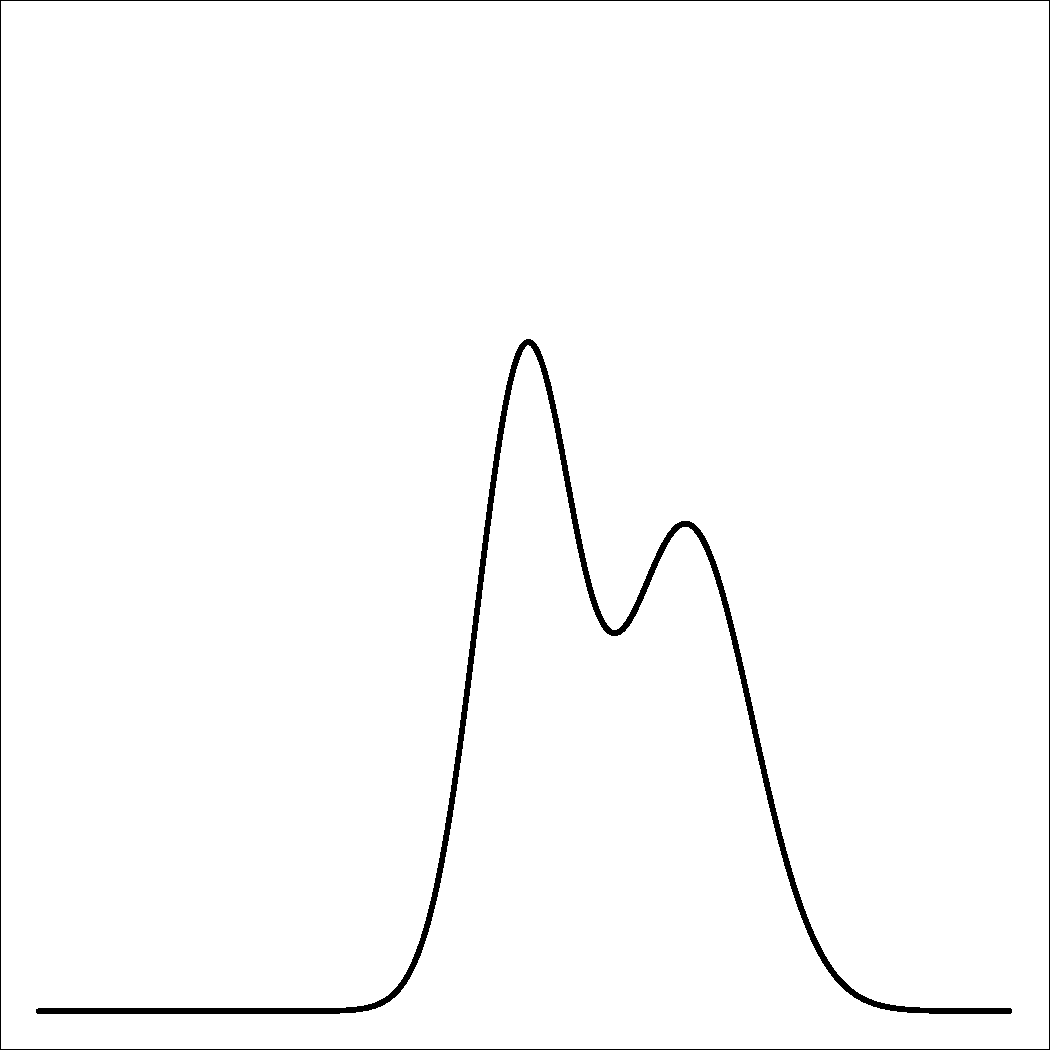
\includegraphics[width=.5\textwidth]{bayesian_update_illustration_th2.pdf}\\
\end{center}
\end{frame}

%----------- slide --------------------------------------------------%
\begin{frame}[t]
  \frametitle{Conceptually, what does solving the summary problem involve?}
  \begin{itemize}
    \item We want to know the distribution from which the dates were generated:
    \pause
    \item A population model
    \pause
    \item End-to-end/aggregate: the fundamental units of inference are "population" models
  \end{itemize}
\end{frame}

%----------- slide --------------------------------------------------%
\begin{frame}[t]
  \frametitle{Fundamental flow of inference: End-to-End}
    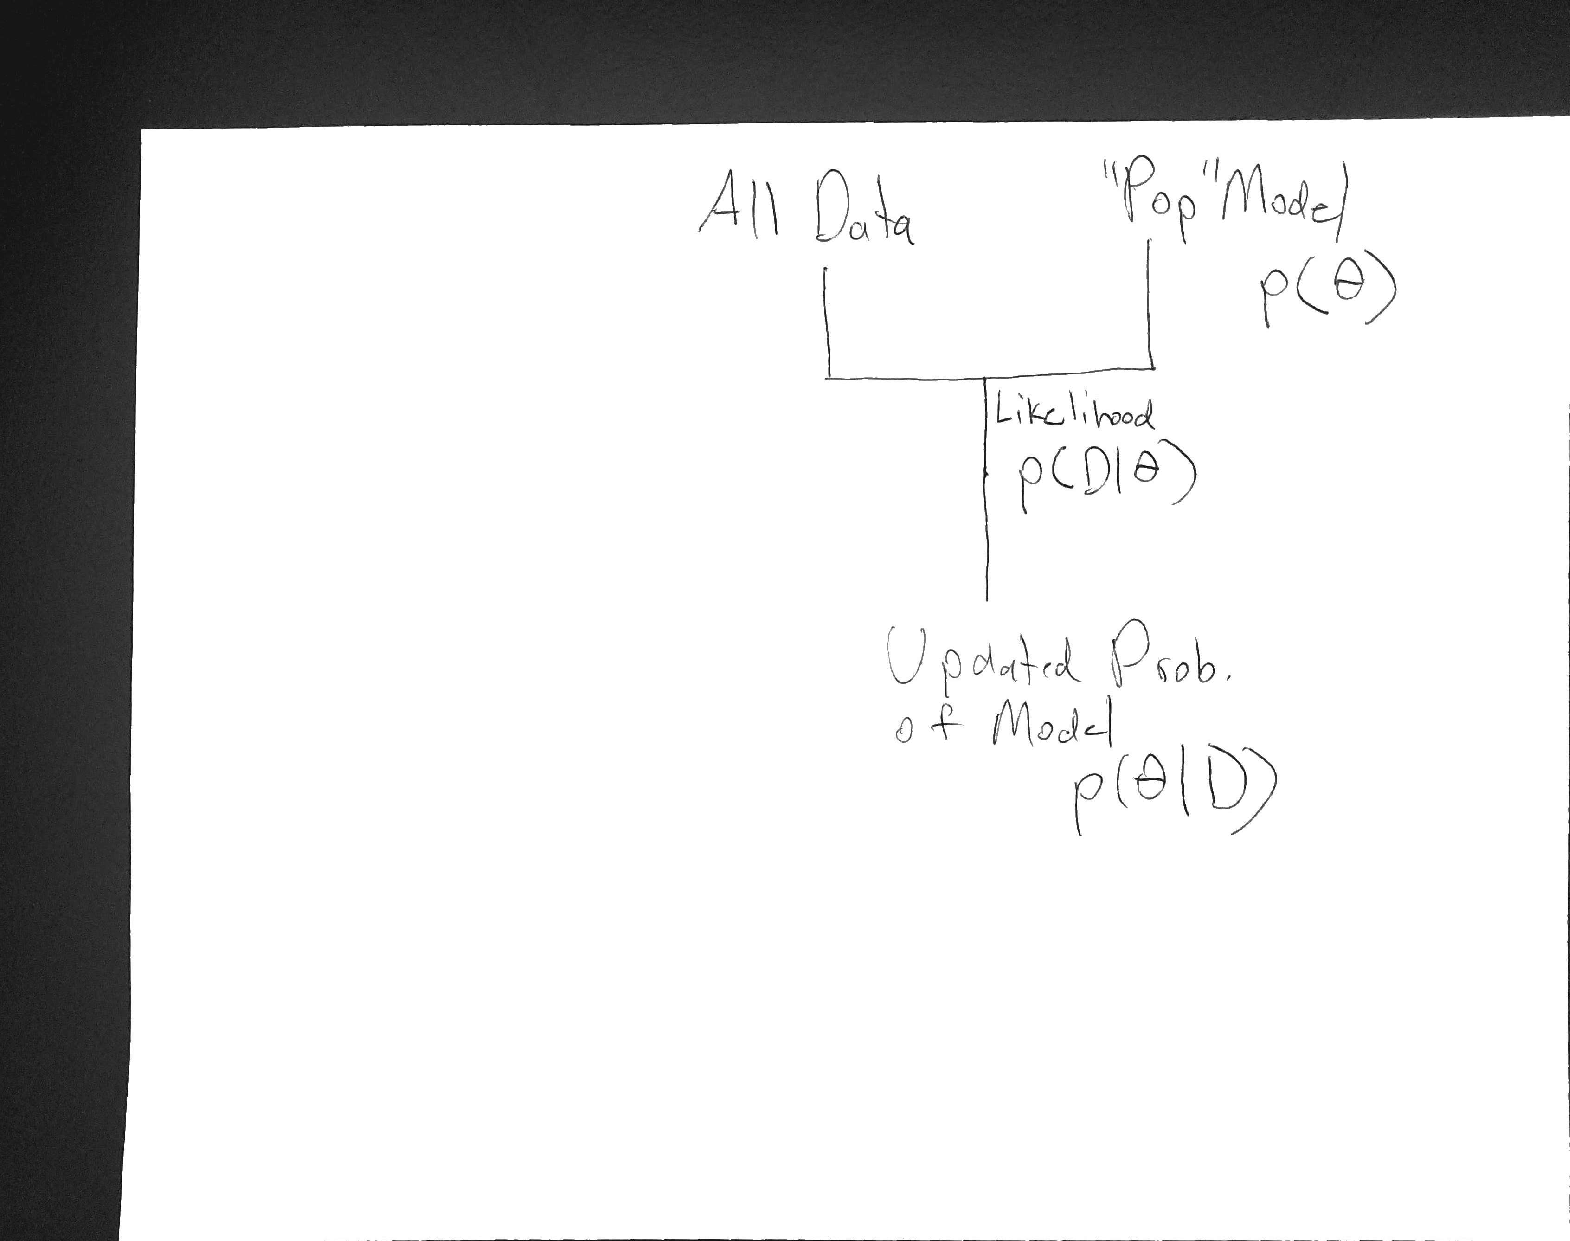
\includegraphics[height=.85\textheight]{e2e_flow.pdf}
\end{frame}

%----------- slide --------------------------------------------------%
\begin{frame}[t]
  \frametitle{Why are SPDs flawed?}
  \begin{itemize}
    \item For SPDs, population models are not the fundamental units of inference
    \pause
    \item Because SPDs involve separate calibrations of each observation, ambiguity from the radiocarbon calibration curve is not dealt with at the aggregate level.
    
    \item SPDs ``conflate process variation and chronological uncertainty'', Carleton and Groucutt (2020)
    
  \end{itemize}
\end{frame}

%----------- slide --------------------------------------------------%
\begin{frame}[t]
  \frametitle{Fundamental flow of inference: SPDs}
    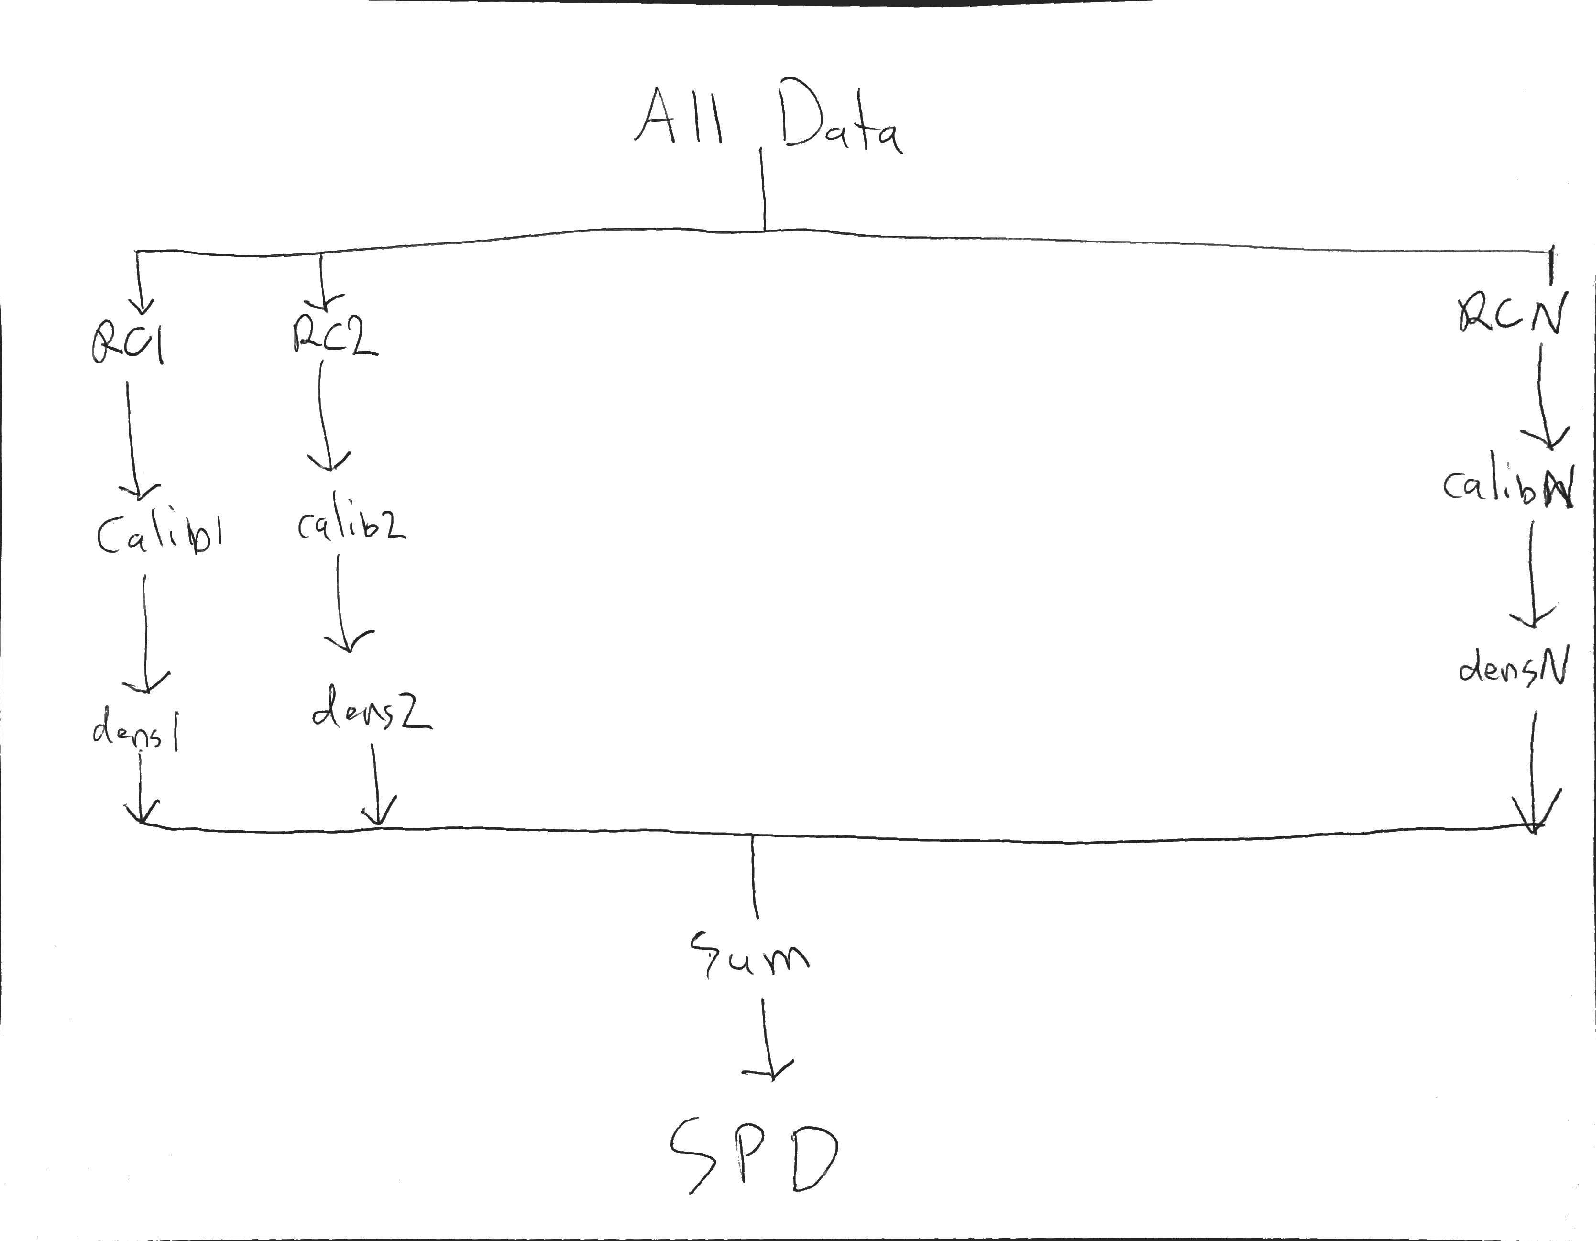
\includegraphics[height=.85\textheight]{spd_flow.pdf}
\end{frame}

%----------- slide --------------------------------------------------%
\begin{frame}[t]
  \frametitle{Fundamental flow of inference: SPDs}
    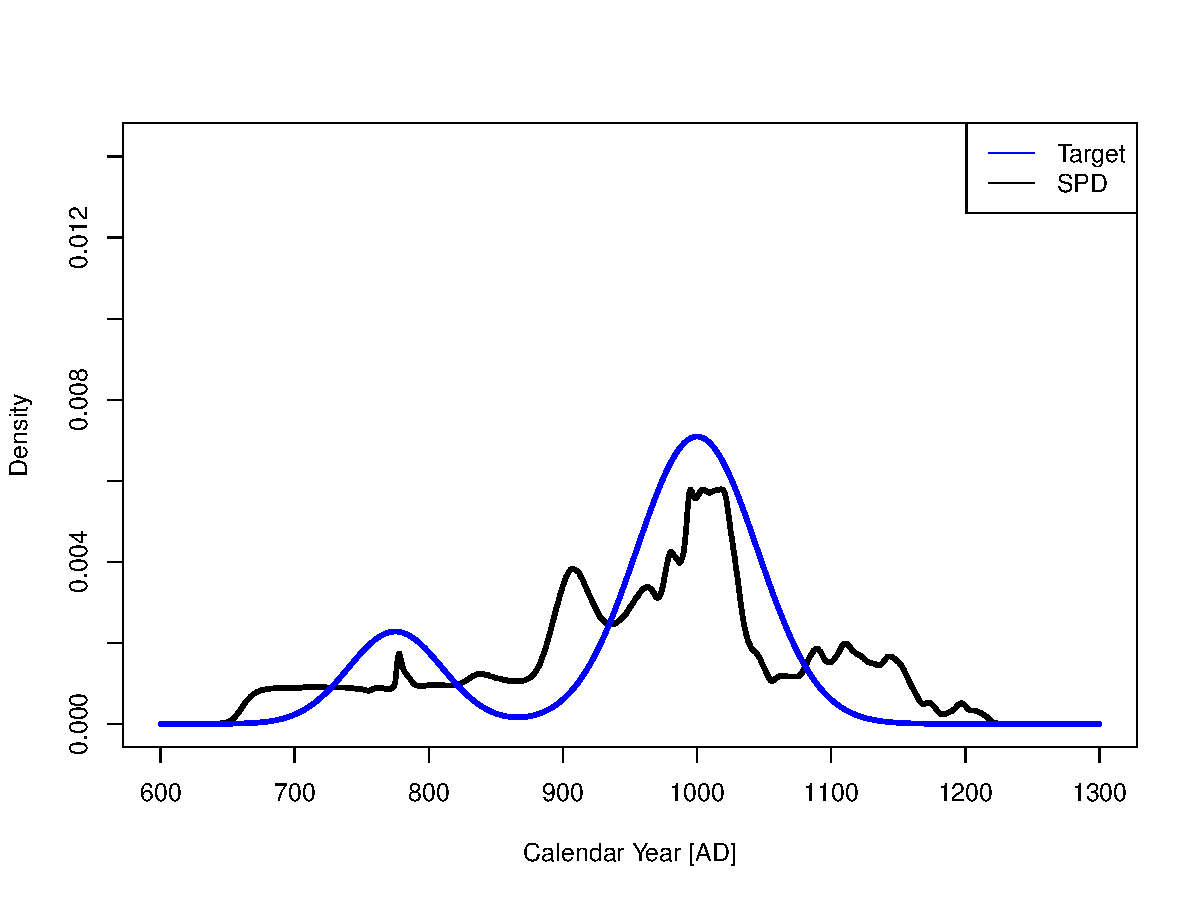
\includegraphics[height=.85\textheight]{sim_spd_10000.pdf}
\end{frame}

%----------- slide --------------------------------------------------%
%\begin{frame}[t]
%    \frametitle{Bayesian Inference}
%    \begin{columns}[c]
%        \column{.333\textwidth}
%            \begin{flushright}
%                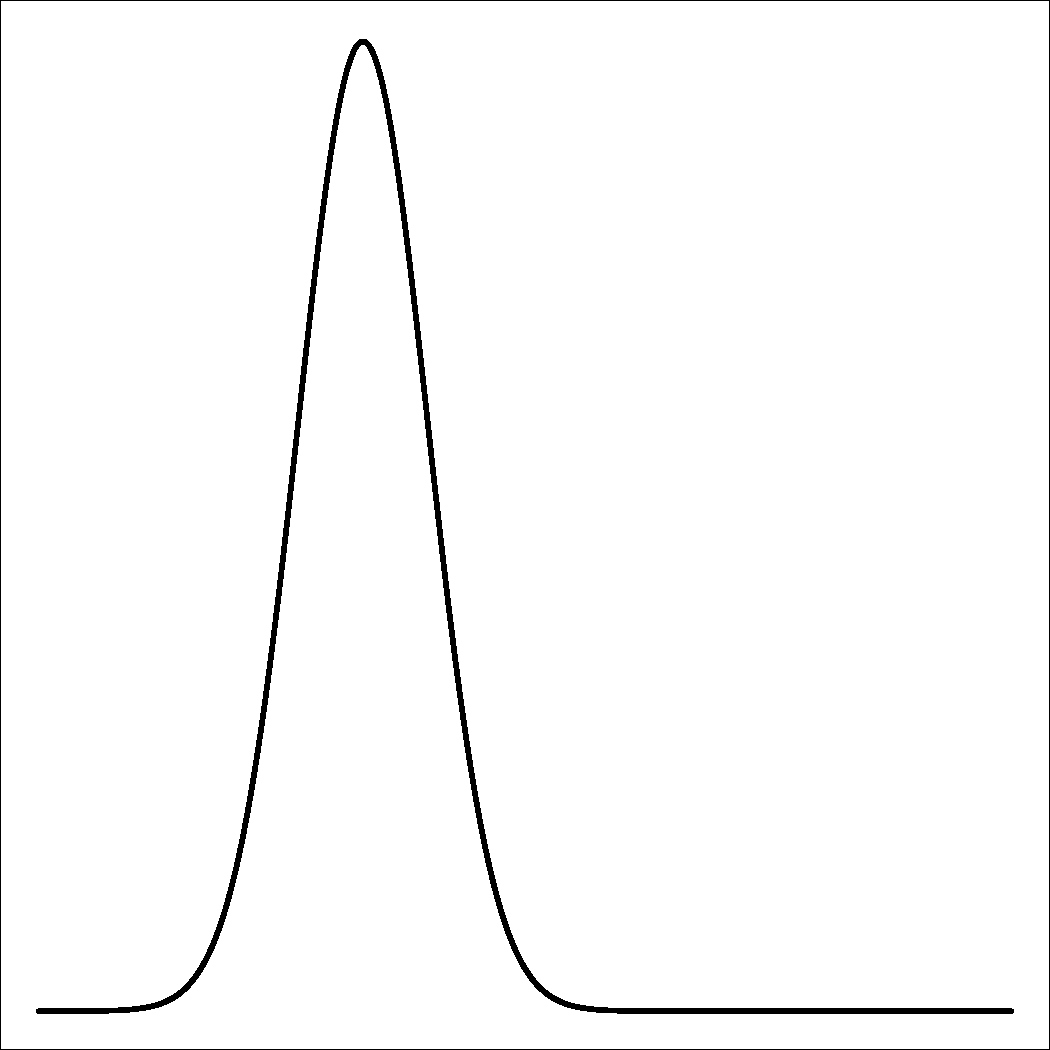
\includegraphics[width=1\textwidth]{bayesian_update_illustration_th1.pdf}
%            \end{flushright}
%        \column{.333\textwidth}
%            \begin{flushright}
%                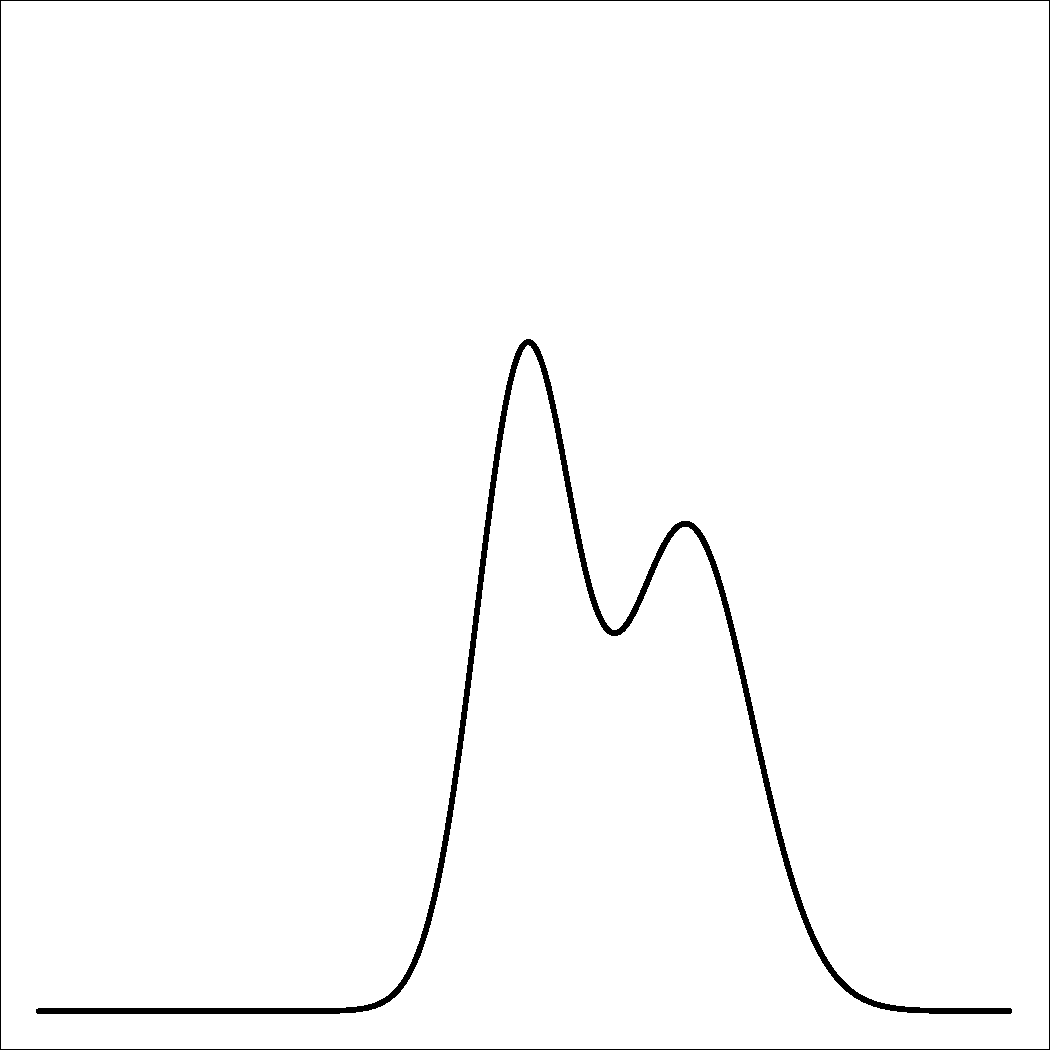
\includegraphics[width=1\textwidth]{bayesian_update_illustration_th2.pdf}
%            \end{flushright}
%        \column{.333\textwidth}
%            \begin{flushright}
%                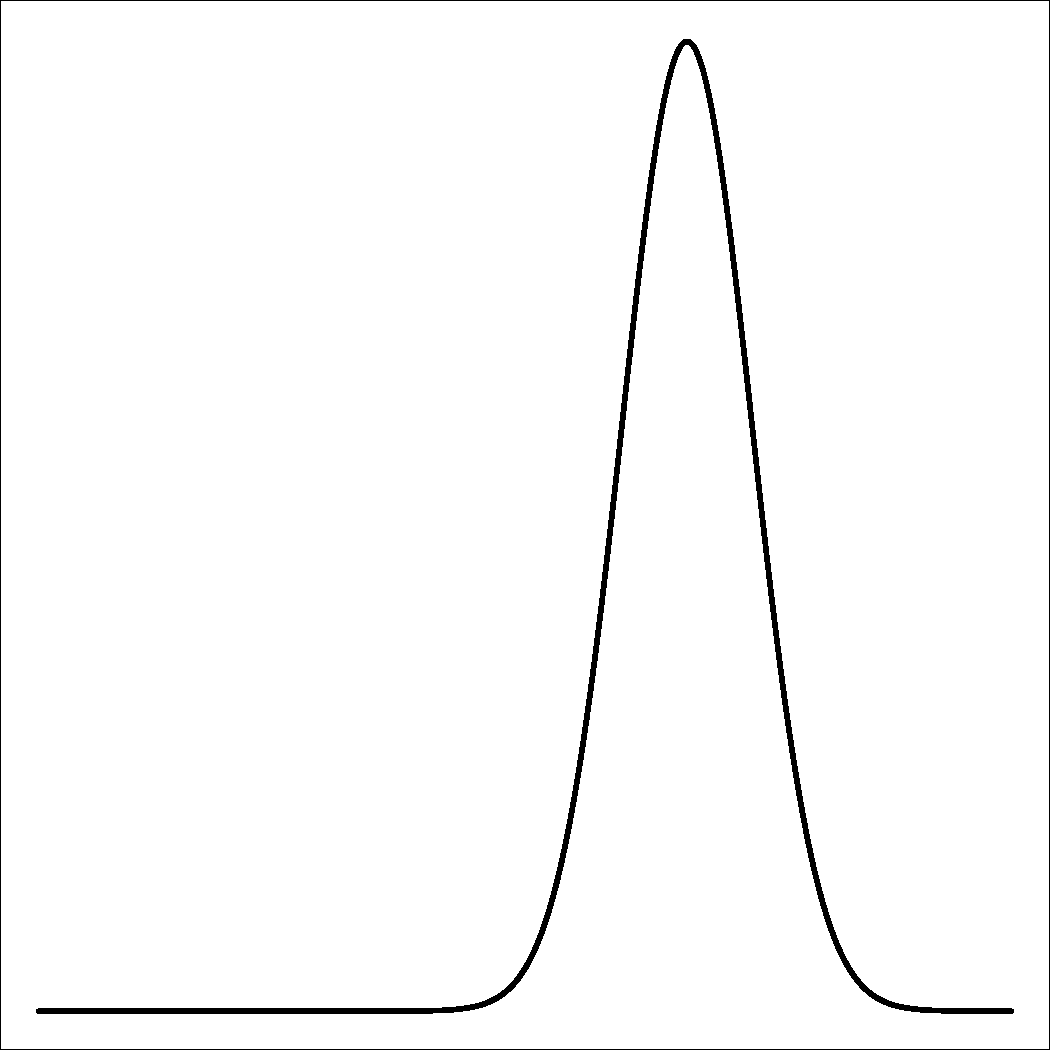
\includegraphics[width=1\textwidth]{bayesian_update_illustration_th3.pdf}
%            \end{flushright}
%    \end{columns}
%\end{frame}

%----------- slide --------------------------------------------------%
%\begin{frame}[t]
%    \frametitle{Bayesian Inference}
%    \begin{columns}[c]
%        \column{.333\textwidth}
%            \begin{flushright}
%                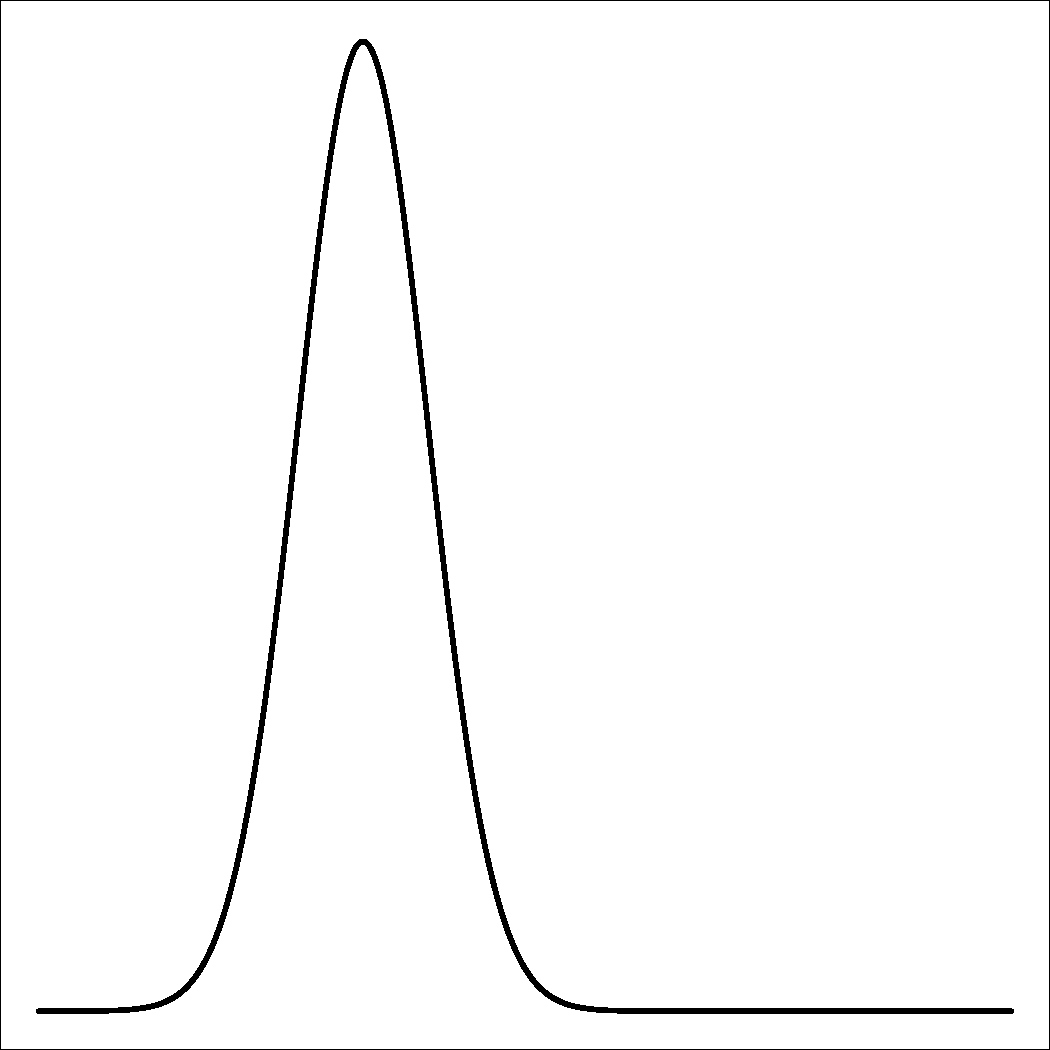
\includegraphics[width=1\textwidth]{bayesian_update_illustration_th1.pdf}\\
%                \vspace{10pt}
%                \Large Prior \hfill $0.40$\\
%            \end{flushright}
%        \column{.333\textwidth}
%            \begin{flushright}
%                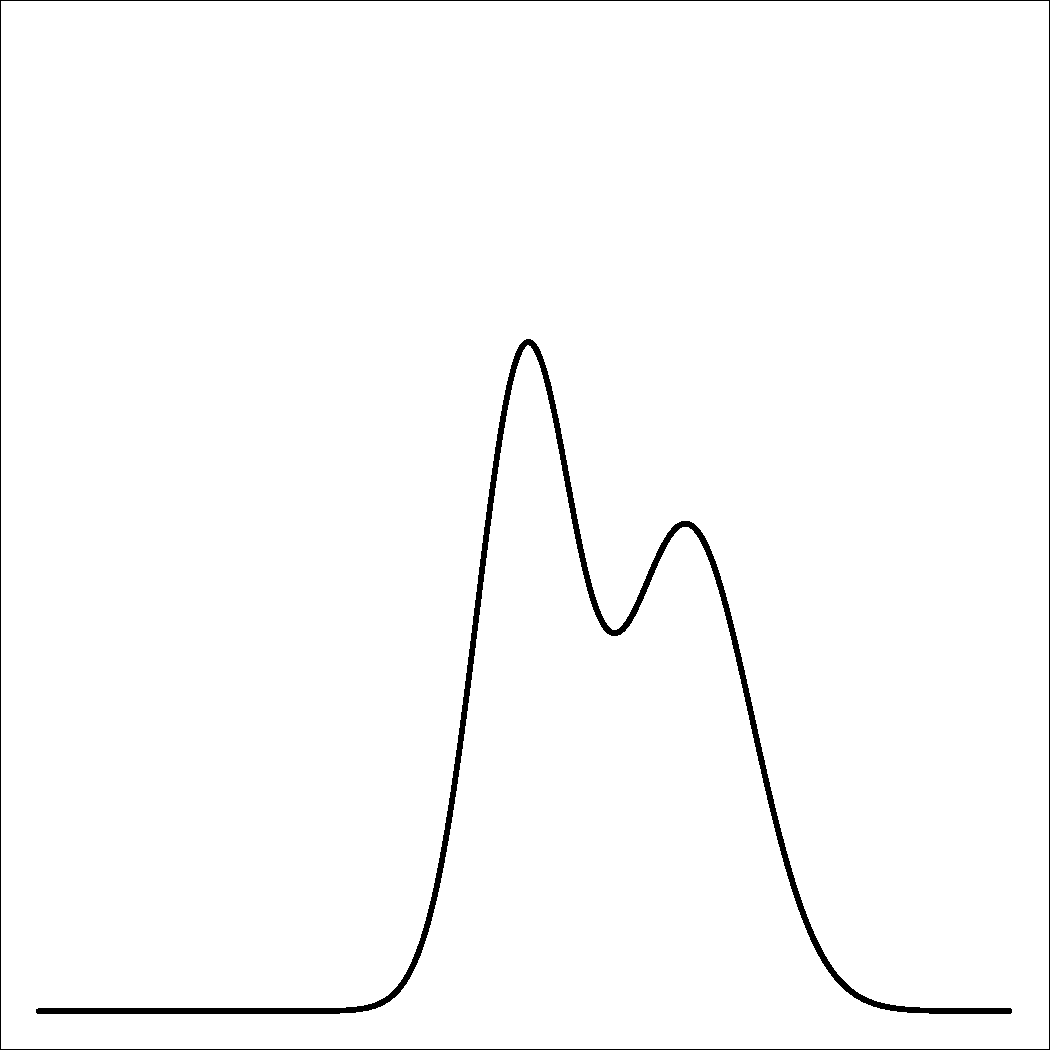
\includegraphics[width=1\textwidth]{bayesian_update_illustration_th2.pdf}\\
%                \vspace{10pt}
%                \Large $0.20$\\
%            \end{flushright}
%        \column{.333\textwidth}
%            \begin{flushright}
%                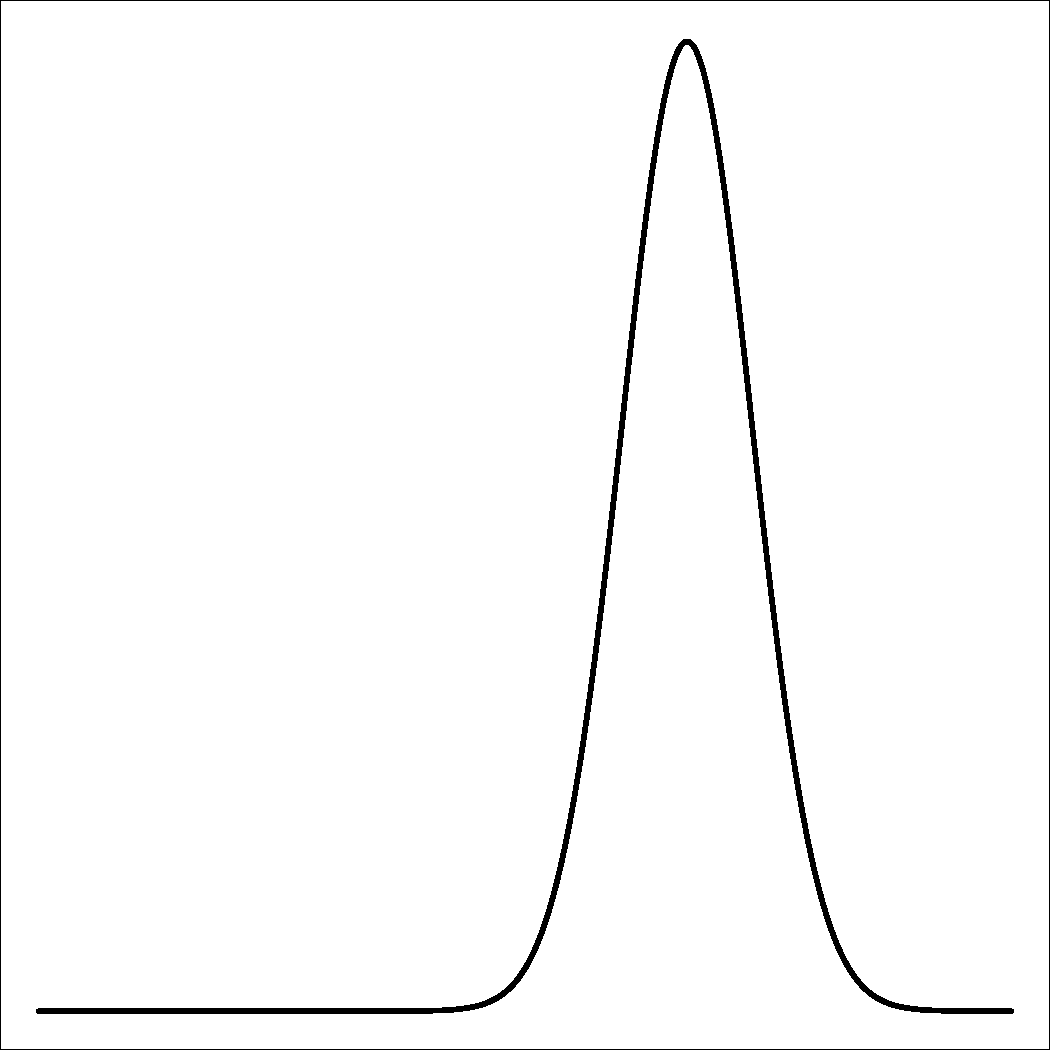
\includegraphics[width=1\textwidth]{bayesian_update_illustration_th3.pdf}\\
%                \vspace{10pt}
%                \Large $0.4$\\
%            \end{flushright}
%    \end{columns}
%\end{frame}

%----------- slide --------------------------------------------------%
%\begin{frame}[t]
%    \frametitle{Bayesian Inference}
%    \begin{columns}[c]
%        \column{.333\textwidth}
%            \begin{flushright}
%                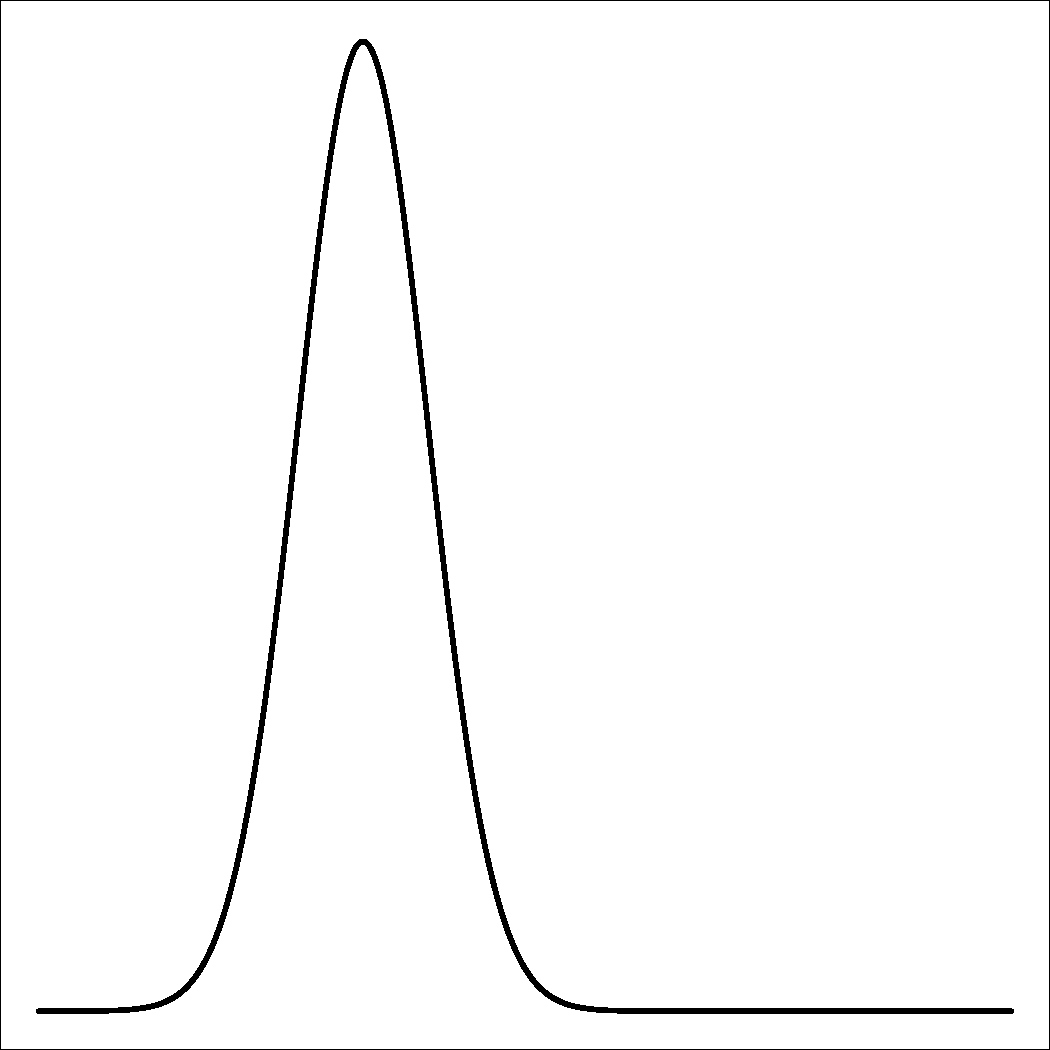
\includegraphics[width=1\textwidth]{bayesian_update_illustration_th1.pdf}\\
%                \vspace{10pt}
%                \Large Prior \hfill $0.40$\\
%                \vspace{20pt}
%                \Large Likelihood \hfill $0.02$\\
%            \end{flushright}
%        \column{.333\textwidth}
%            \begin{flushright}
%                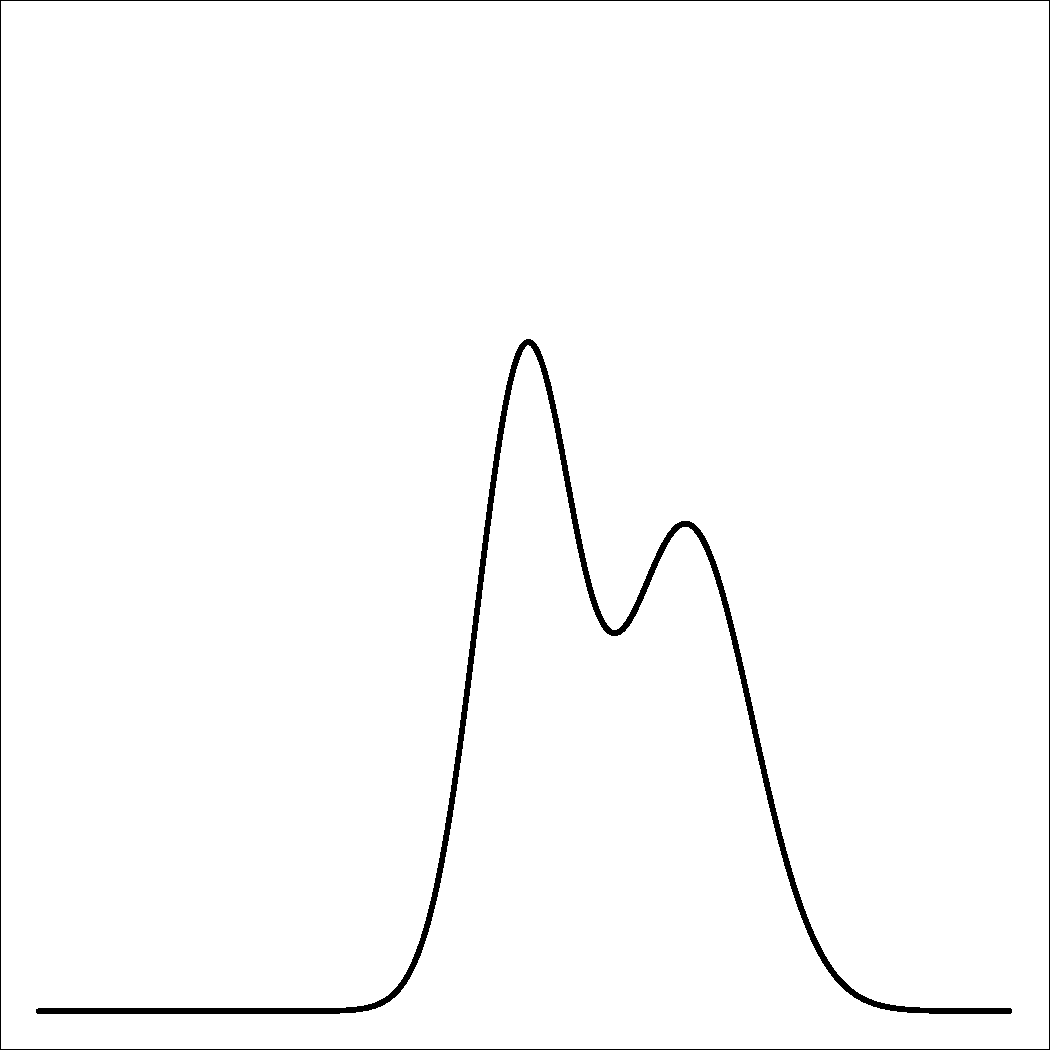
\includegraphics[width=1\textwidth]{bayesian_update_illustration_th2.pdf}\\
%                \vspace{10pt}
%                \Large $0.20$\\
%                \vspace{20pt}
%                \Large $1.00$\\
%            \end{flushright}
%        \column{.333\textwidth}
%            \begin{flushright}
%                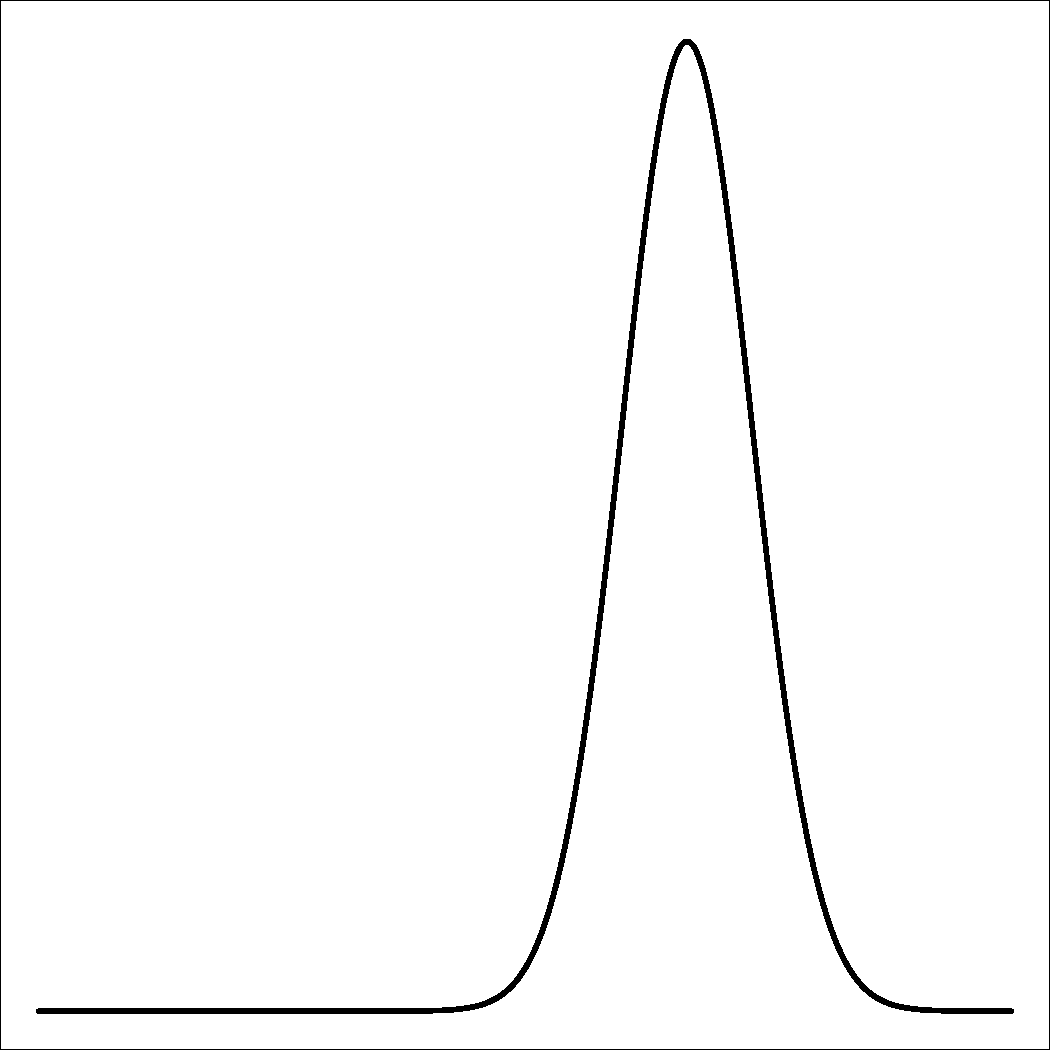
\includegraphics[width=1\textwidth]{bayesian_update_illustration_th3.pdf}\\
%                \vspace{10pt}
%                \Large $0.4$\\
%                \vspace{20pt}
%                \Large $0.04$\\
%            \end{flushright}
%    \end{columns}
%\end{frame}

%----------- slide --------------------------------------------------%
%\begin{frame}[t]
%    \frametitle{Bayesian Inference}
%    \begin{columns}[c]
%        \column{.333\textwidth}
%            \begin{flushright}
%                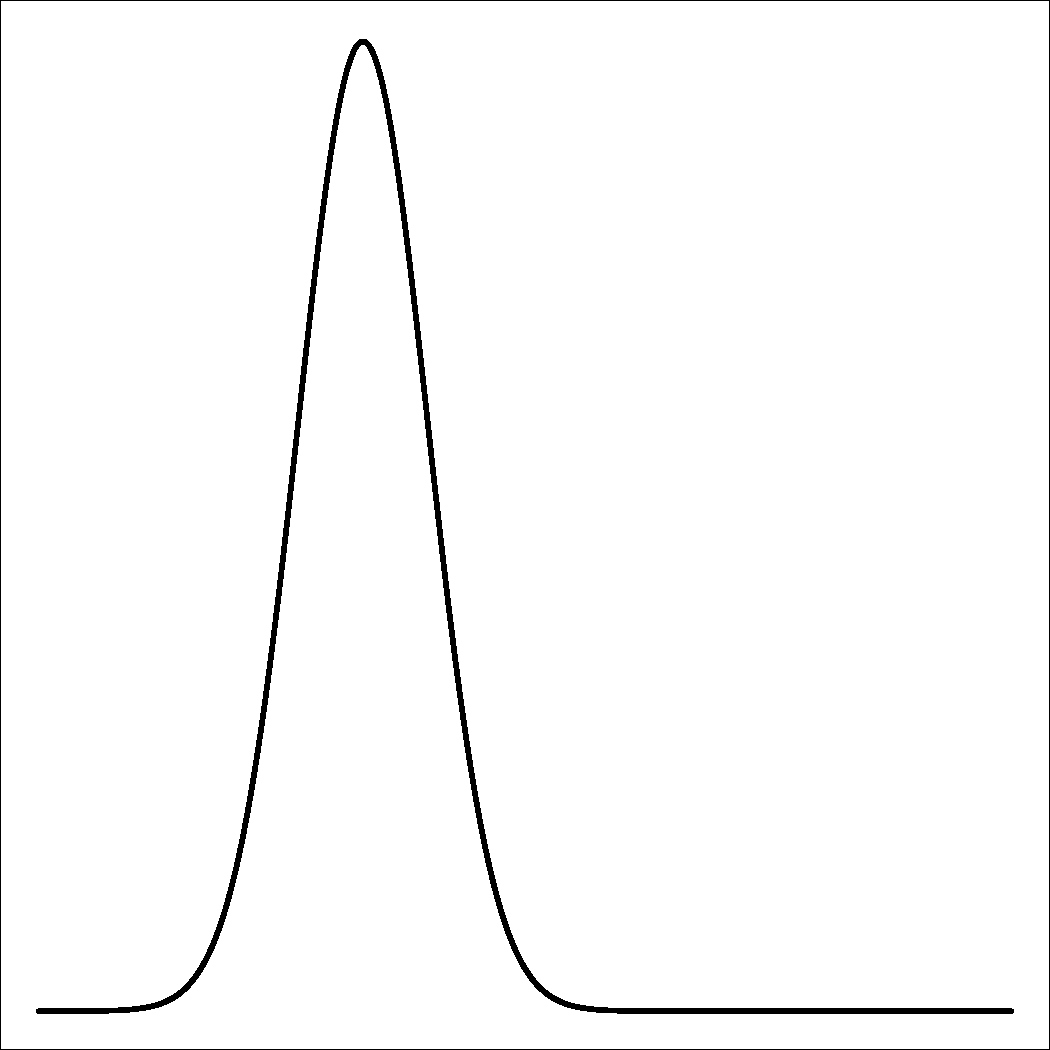
\includegraphics[width=1\textwidth]{bayesian_update_illustration_th1.pdf}\\
%                \vspace{10pt}
%                \Large Prior \hfill $0.40$\\
%                \vspace{20pt}
%                \Large Likelihood \hfill $0.02$\\
%                \vspace{20pt}
%                \Large Posterior \hfill $0.02$
%            \end{flushright}
%        \column{.333\textwidth}
%            \begin{flushright}
%                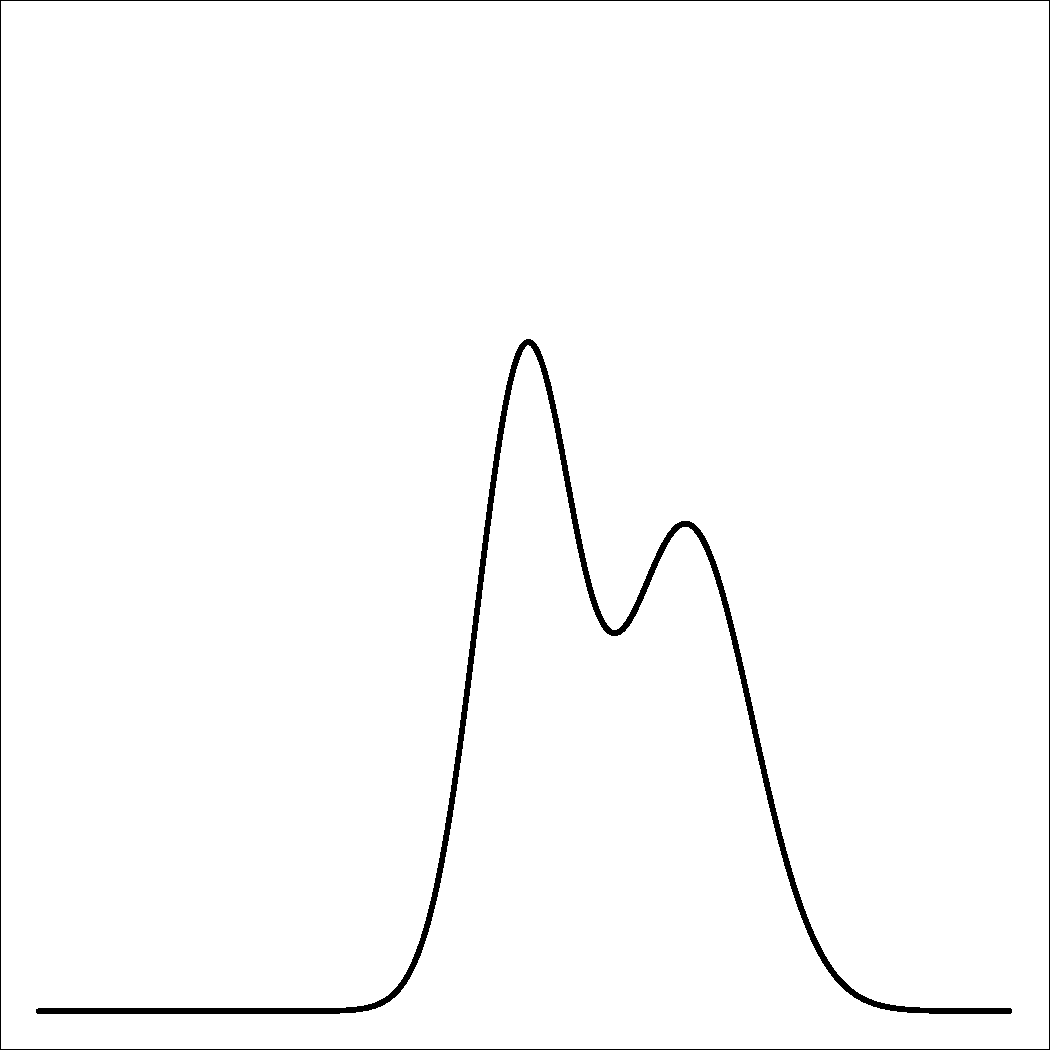
\includegraphics[width=1\textwidth]{bayesian_update_illustration_th2.pdf}\\
%                \vspace{10pt}
%                \Large $0.20$\\
%                \vspace{20pt}
%                \Large $1.00$\\
%                \vspace{20pt}
%                \Large $0.94$
%            \end{flushright}
%        \column{.333\textwidth}
%            \begin{flushright}
%                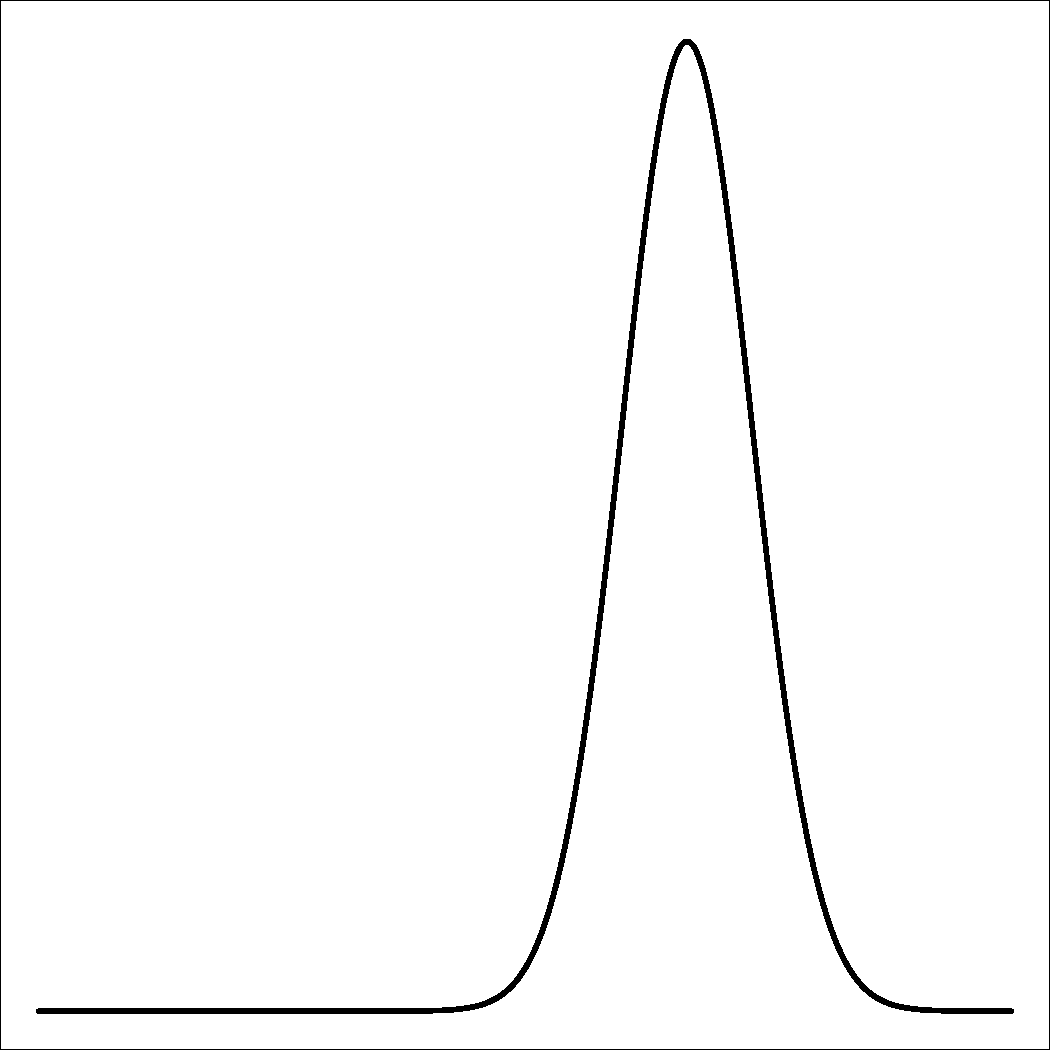
\includegraphics[width=1\textwidth]{bayesian_update_illustration_th3.pdf}\\
%                \vspace{10pt}
%                \Large $0.4$\\
%                \vspace{20pt}
%                \Large $0.04$\\
%                \vspace{20pt}
%                \Large $0.04$
%            \end{flushright}
%    \end{columns}
%\end{frame}

%----------- slide --------------------------------------------------%
%\begin{frame}[t]
%    \frametitle{Bayesian Inference}
%    \begin{columns}[c]
%        \column{.333\textwidth}
%            \begin{flushright}
%                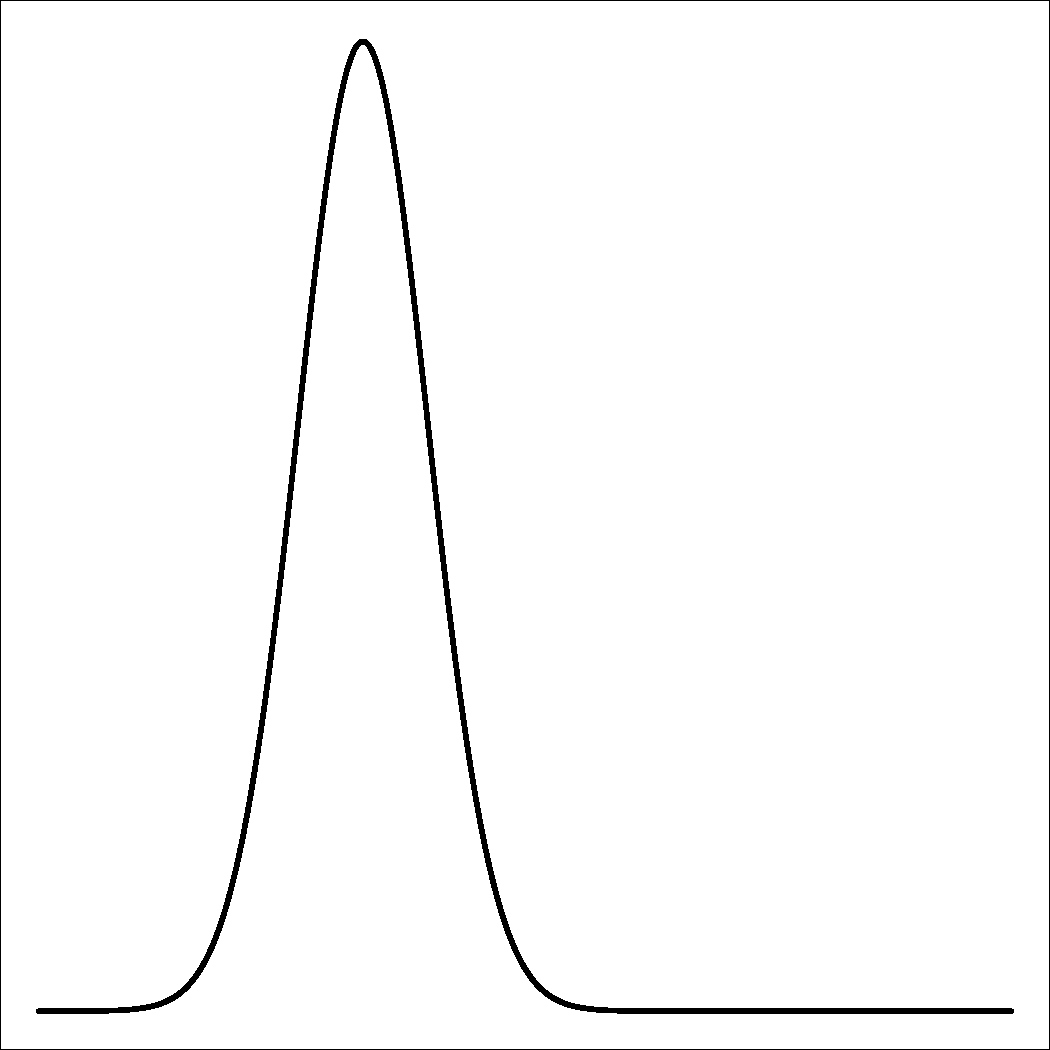
\includegraphics[width=1\textwidth]{bayesian_update_illustration_th1.pdf}\\
%                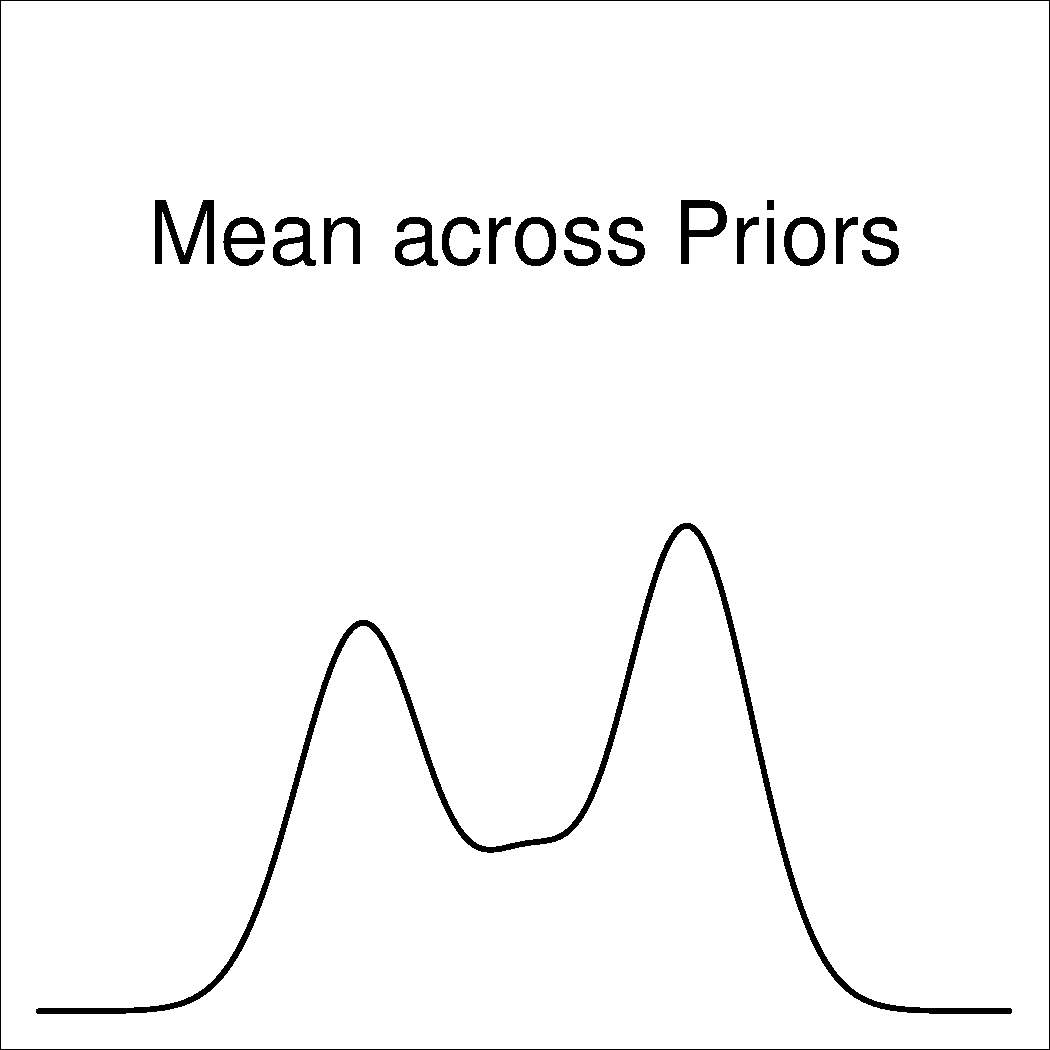
\includegraphics[width=1\textwidth]{bayesian_update_illustration_prior.pdf}\\
%            \end{flushright}
%        \column{.333\textwidth}
%            \begin{flushright}
%                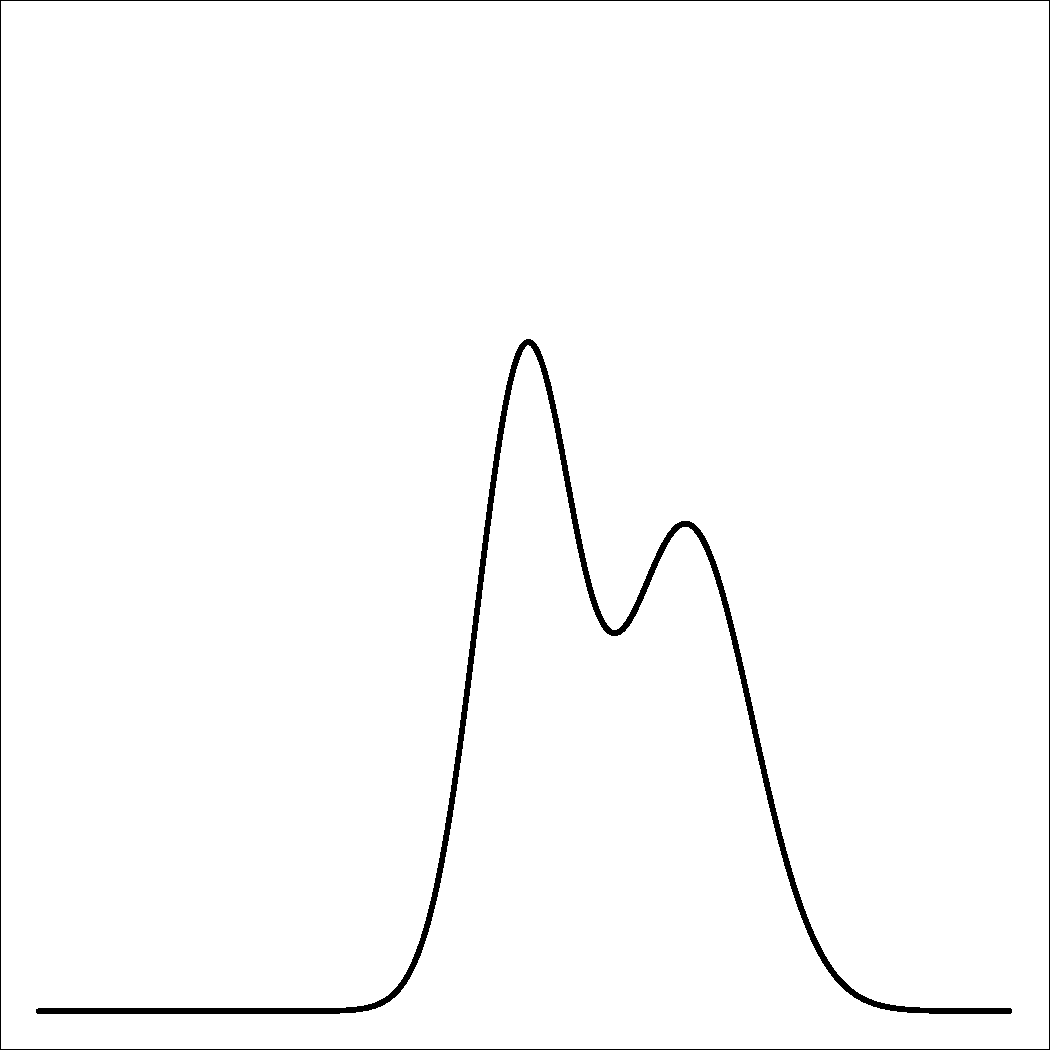
\includegraphics[width=1\textwidth]{bayesian_update_illustration_th2.pdf}\\
%                
\includegraphics[width=1\textwidth]{bayesian_update_illustration_blank.pdf}\\
%            \end{flushright}
%        \column{.333\textwidth}
%            \begin{flushright}
%                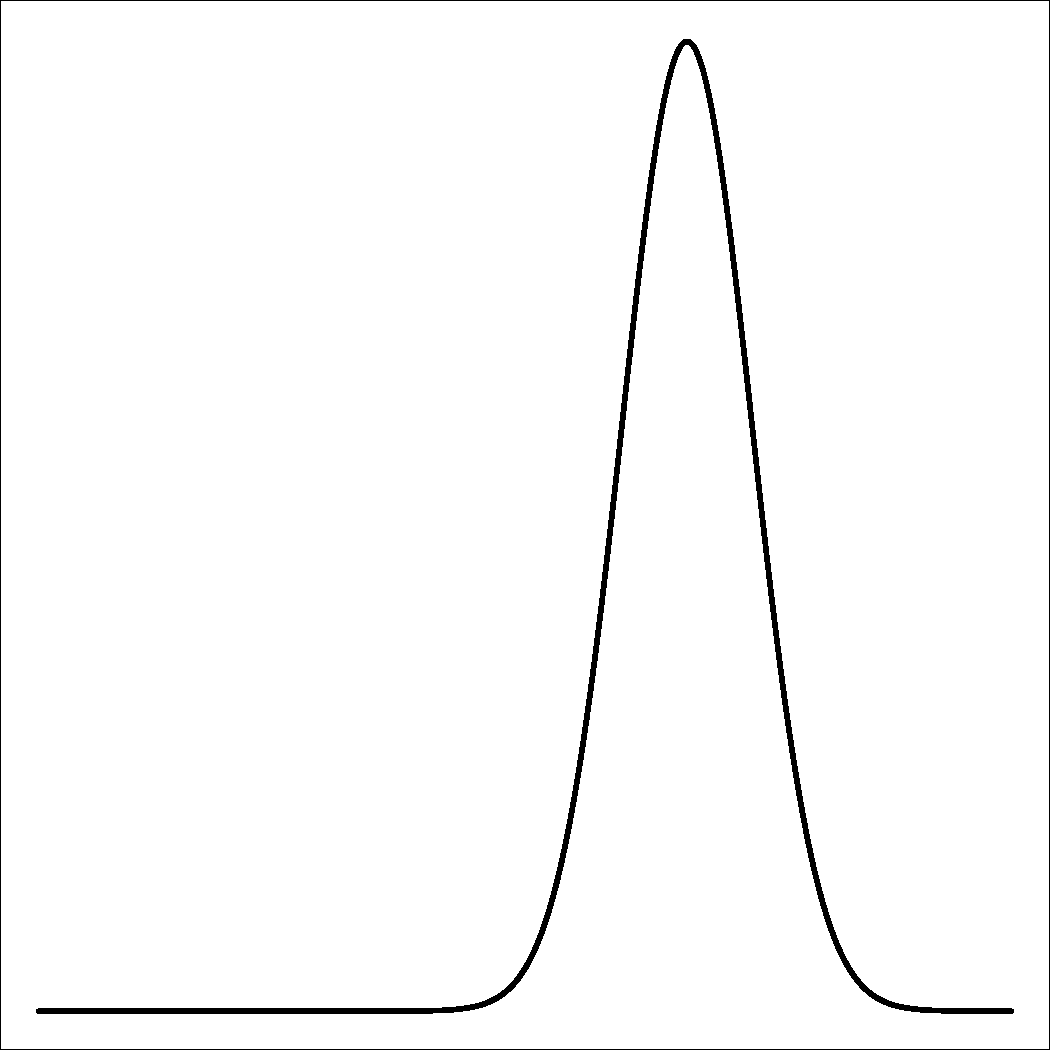
\includegraphics[width=1\textwidth]{bayesian_update_illustration_th3.pdf}\\
%                
\includegraphics[width=1\textwidth]{bayesian_update_illustration_blank.pdf}\\
%            \end{flushright}
%    \end{columns}
%\end{frame}

%----------- slide --------------------------------------------------%
%\begin{frame}[t]
%    \frametitle{Bayesian Inference}
%    \begin{columns}[c]
%        \column{.333\textwidth}
%            \begin{flushright}
%                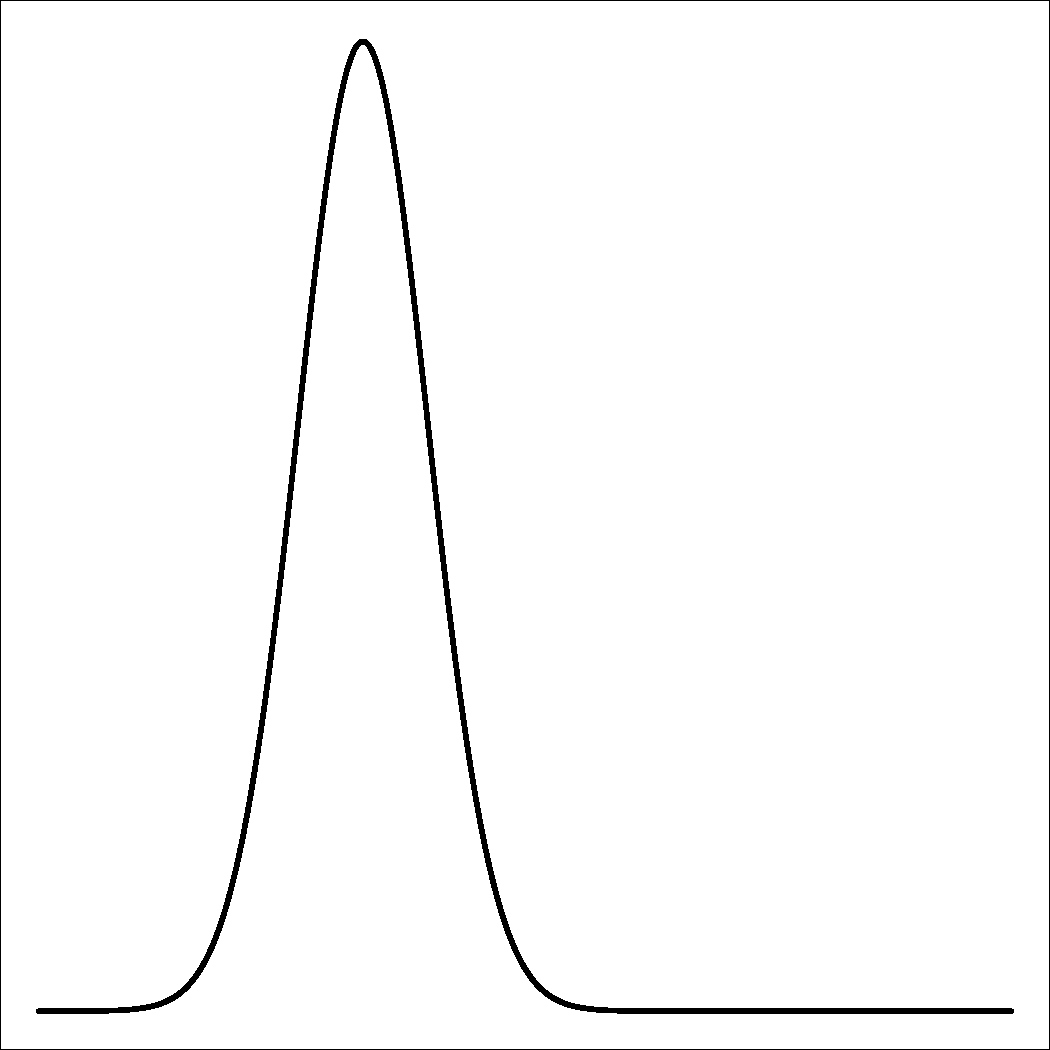
\includegraphics[width=1\textwidth]{bayesian_update_illustration_th1.pdf}\\
%                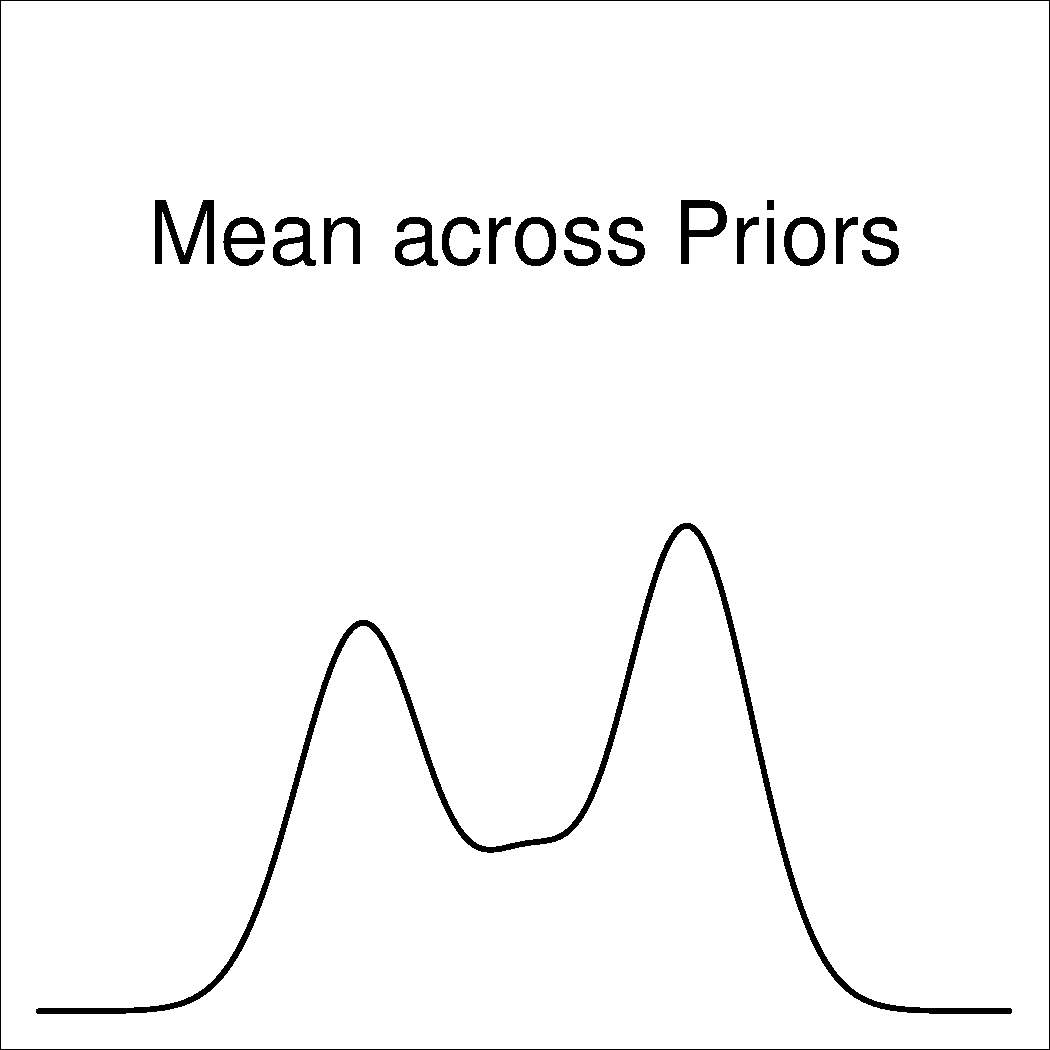
\includegraphics[width=1\textwidth]{bayesian_update_illustration_prior.pdf}\\
%            \end{flushright}
%        \column{.333\textwidth}
%            \begin{flushright}
%                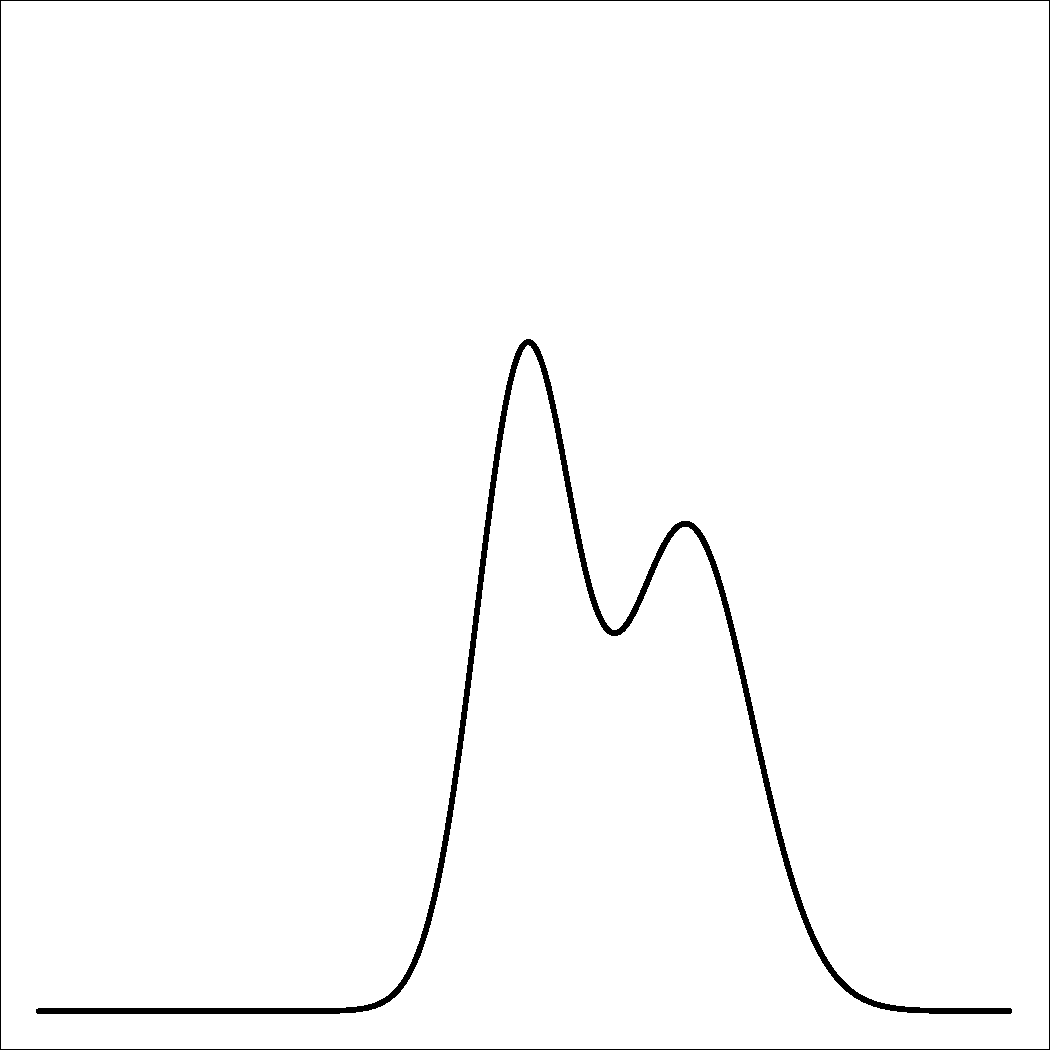
\includegraphics[width=1\textwidth]{bayesian_update_illustration_th2.pdf}\\
%                
\includegraphics[width=1\textwidth]{bayesian_update_illustration_blank.pdf}\\
%            \end{flushright}
%        \column{.333\textwidth}
%            \begin{flushright}
%                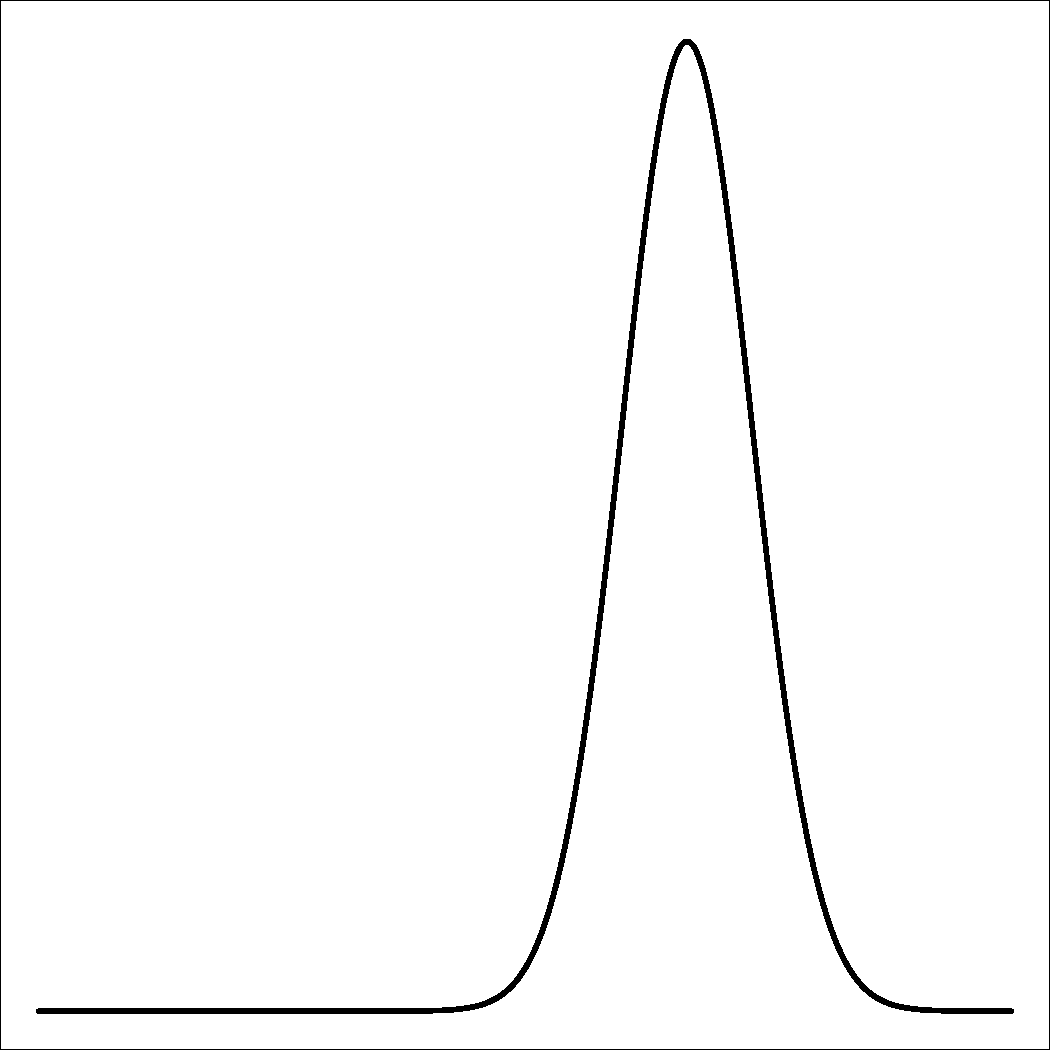
\includegraphics[width=1\textwidth]{bayesian_update_illustration_th3.pdf}\\
%                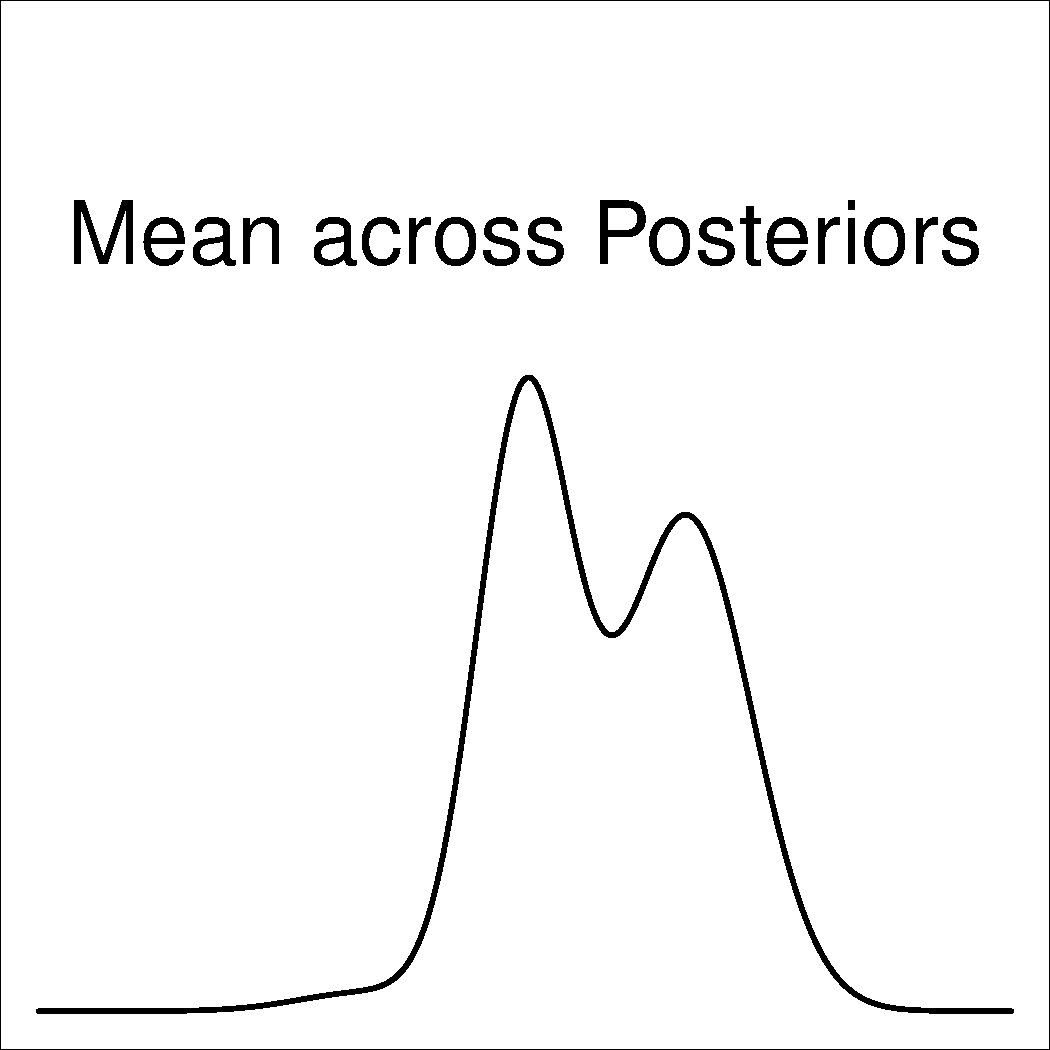
\includegraphics[width=1\textwidth]{bayesian_update_illustration_posterior.pdf}\\
%            \end{flushright}
%    \end{columns}
%\end{frame}

%----------- slide --------------------------------------------------%
\begin{frame}[t]
  \frametitle{A simulation}
    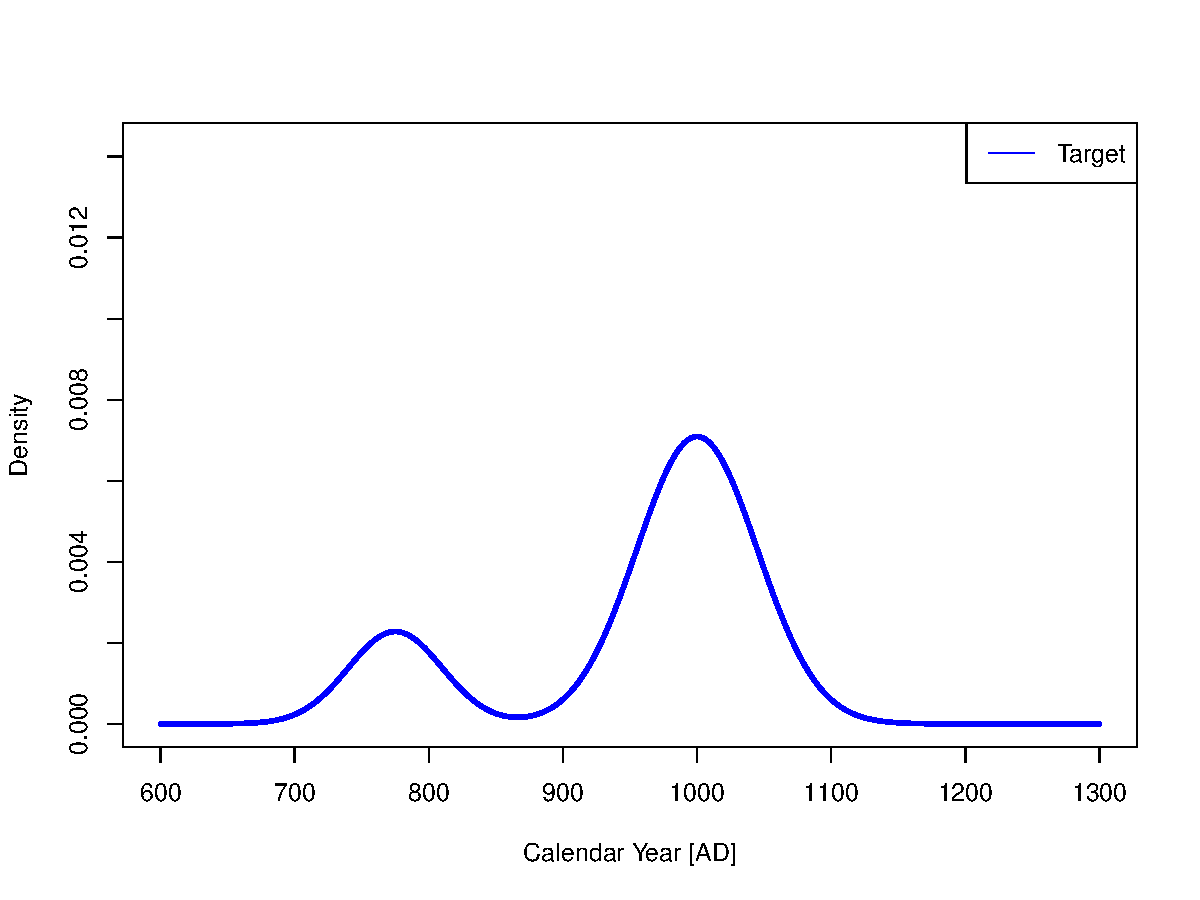
\includegraphics[height=.85\textheight]{sim_target.pdf}
\end{frame}

%----------- slide --------------------------------------------------%
\begin{frame}[t]
  \frametitle{A simulation [N=10000]}
    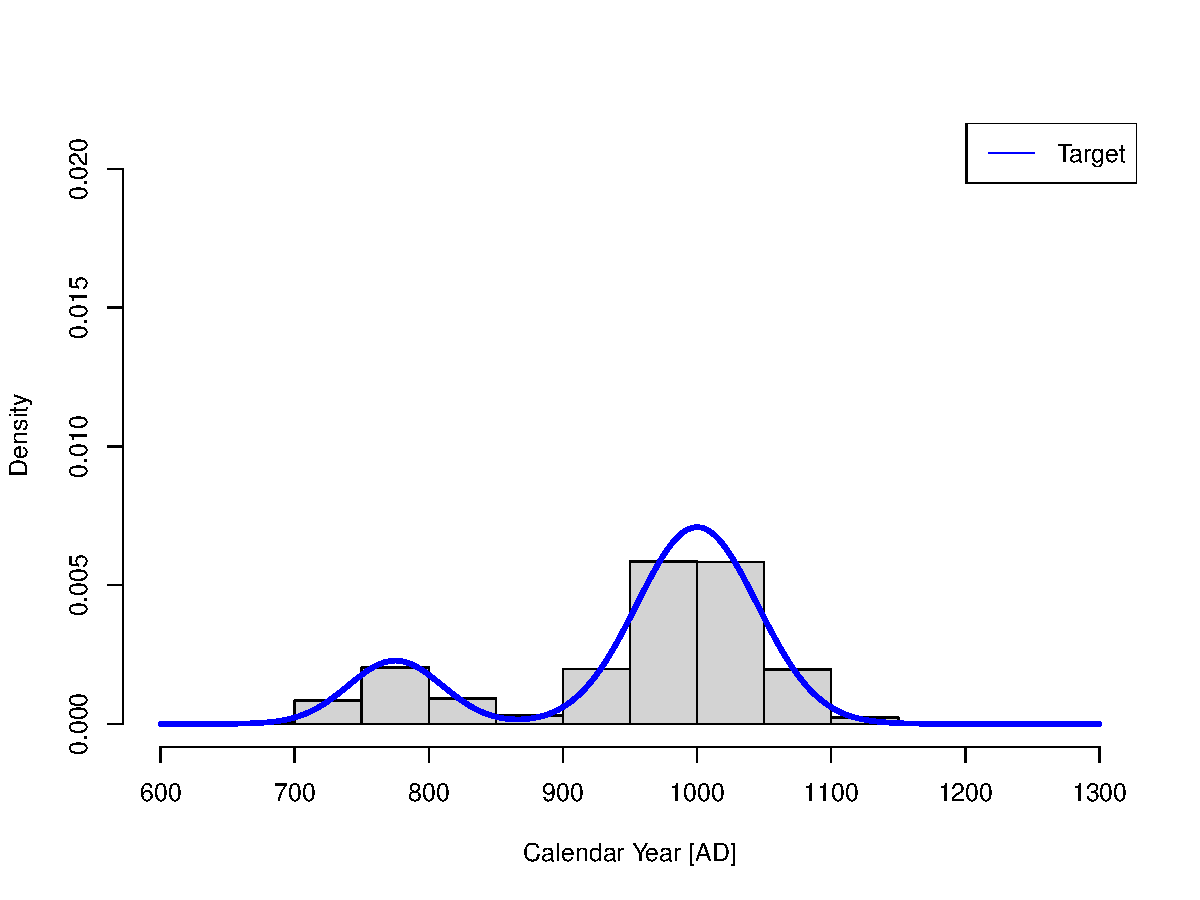
\includegraphics[height=.85\textheight]{sim_target_with_hist.pdf}
\end{frame}

%----------- slide --------------------------------------------------%
\begin{frame}[t]
  \frametitle{A simulation [N=10000]}
    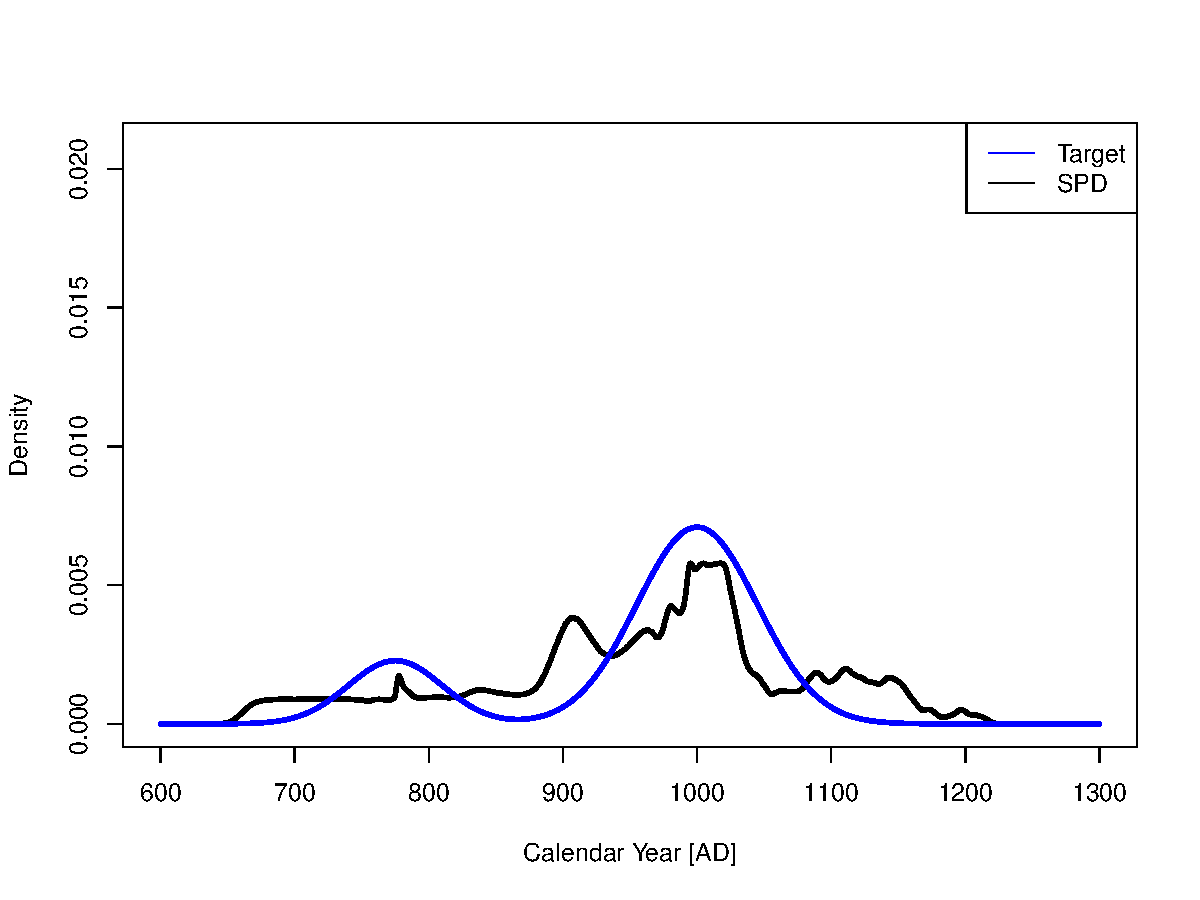
\includegraphics[height=.85\textheight]{sim_target_spd_10000.pdf}
\end{frame}

%----------- slide --------------------------------------------------%
\begin{frame}[t]
  \frametitle{A simulation [N=10000]}
    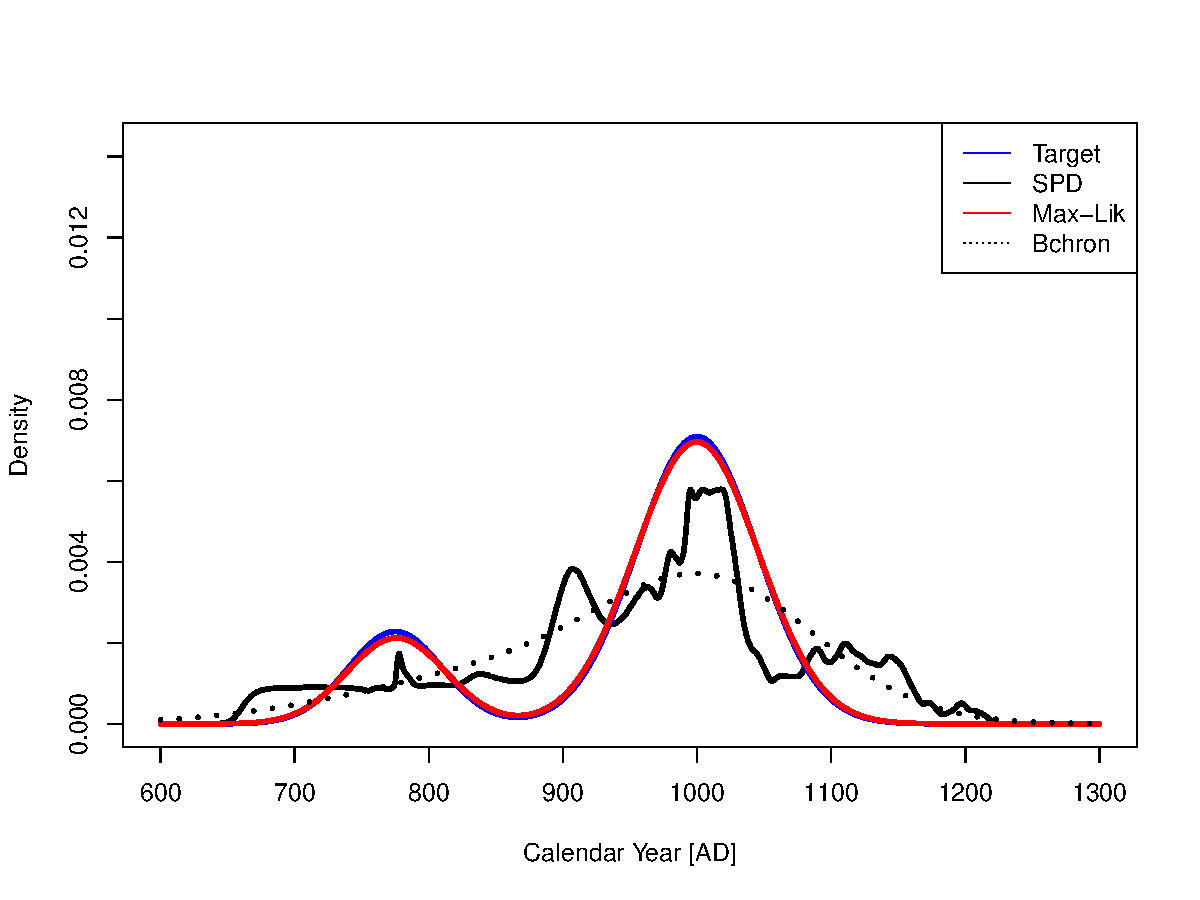
\includegraphics[height=.85\textheight]{sim_target_spd_max-lik_bchron_10000.pdf}
\end{frame}

%----------- slide --------------------------------------------------%
\begin{frame}[t]
  \frametitle{A simulation [N=100]}
    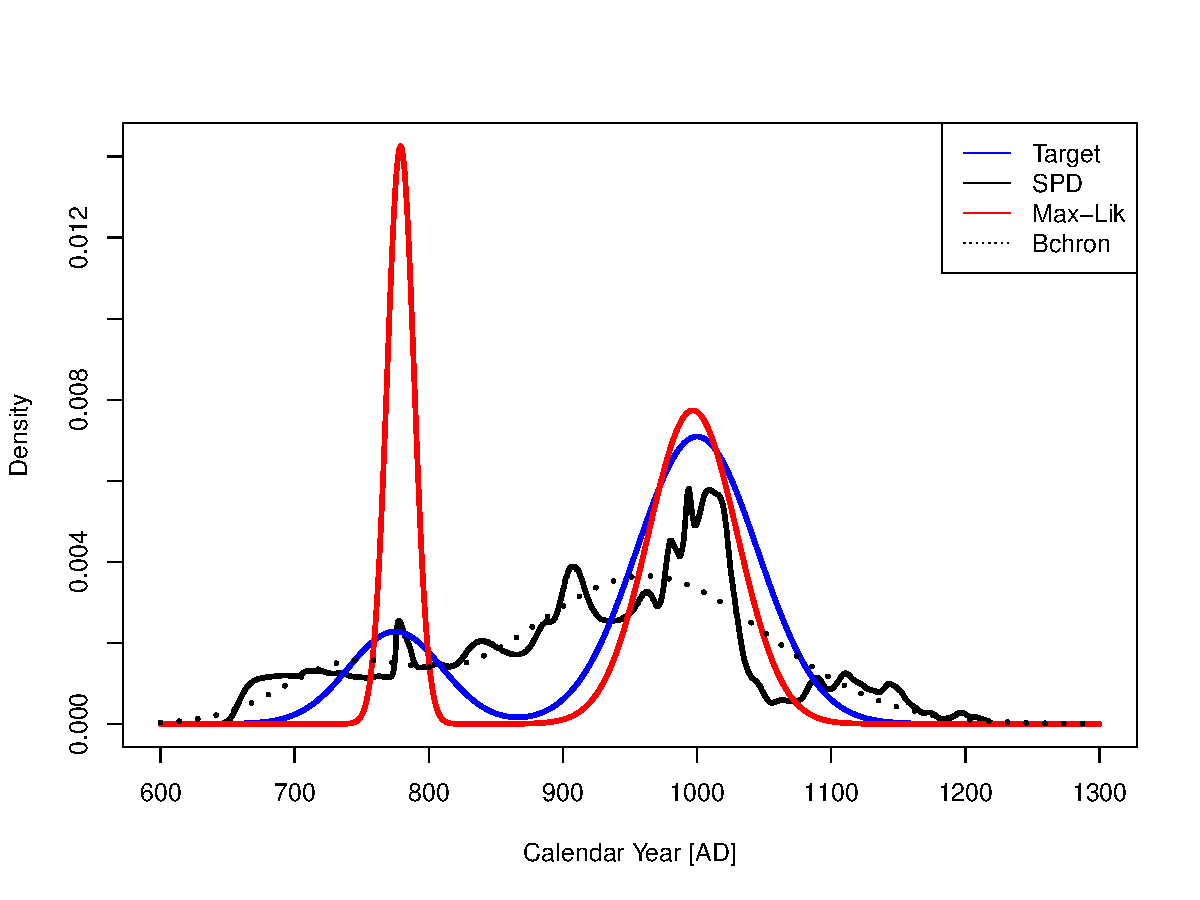
\includegraphics[height=.85\textheight]{sim_target_spd_max-lik_bchron_100.pdf}
\end{frame}

%----------- slide --------------------------------------------------%
\begin{frame}[t]
  \frametitle{A simulation [N=1000]}
    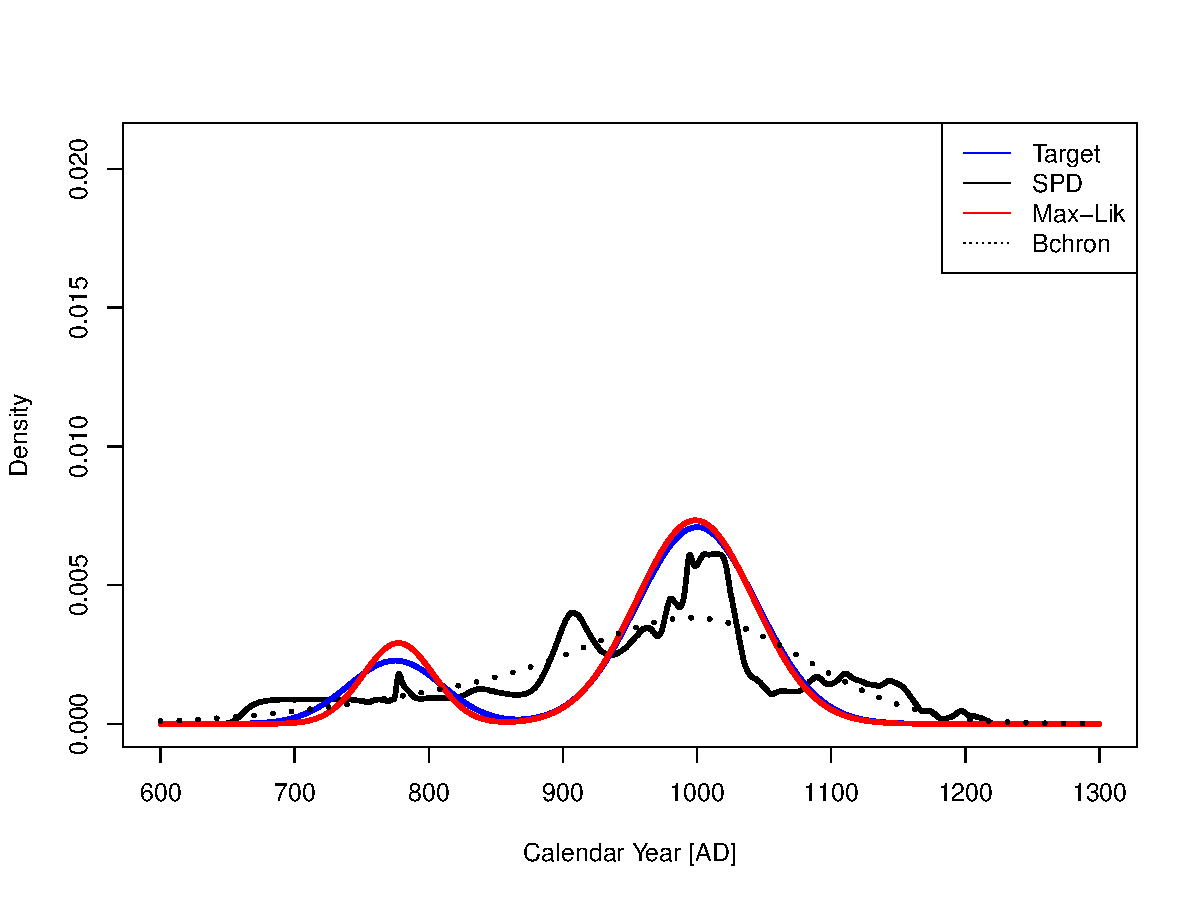
\includegraphics[height=.85\textheight]{sim_target_spd_max-lik_bchron_1000.pdf}
\end{frame}

%----------- slide --------------------------------------------------%
\begin{frame}[t]
  \frametitle{Simulation with Bayesian Inference}
    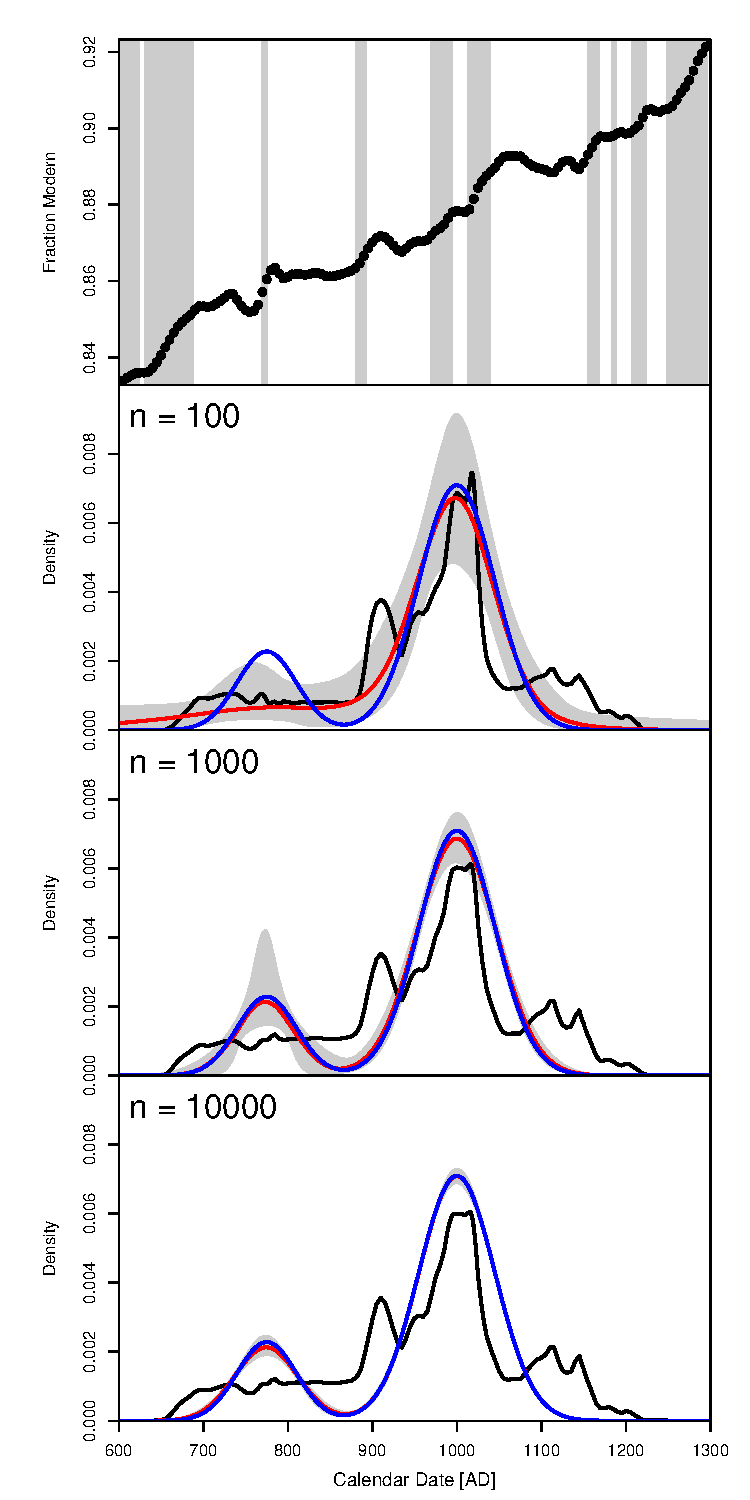
\includegraphics[height=.85\textheight]{Fig1_sim_inference.pdf}
\end{frame}

%----------- slide --------------------------------------------------%
\begin{frame}[c]
  \frametitle{Recent work outside the SPD+ realm}
    \begin{itemize}
      \item Price et al. (2020; biorxiv) -- End-to-end Bayesian analysis of 14C dates reveals new insights into lowland Maya demography
      \item Carleton 2020 -- Evaluating Bayesian Radiocarbon-dated Event Count (REC) models for the study of long-term human and environmental processes
      \item Carleton and Groucutt 2020 -- Sum things are not what they seem
      \item Timpson et al. 2020 -- Directly modelling population dynamics in the South American Arid Diagonal using 14C dates
  \end{itemize}
\end{frame}

%----------- slide --------------------------------------------------%
\begin{frame}[t]
  \frametitle{Relevant Data}
  \begin{columns}[c]
   \column{.5\textwidth}
     \begin{block}{Direct}
     \begin{itemize}
       \pause
       \item{Date of Death [C14]} 
       \pause
       \item{Age at Death} 
       \pause
       \item{Isotopes} 
       \pause
       \item{DNA} 
     \end{itemize}
     \end{block}
    \pause

    \column{.5\textwidth}
     \begin{block}{Indirect}
     \begin{itemize}
       \pause
       \item{Pottery} 
       \pause
       \item{Charcoal} 
       \pause
       \item{House Counts} 
       \pause
       \item{etc.} 
     \end{itemize}
     \end{block}
  \end{columns}
\end{frame}

%----------- slide --------------------------------------------------%
\begin{frame}[c]
    \frametitle{The Team}
    \begin{itemize}
      \item José M. Capriles
      \item Julie A. Hoggarth
      \item R. Kyle Bocinsky
      \item Claire E. Ebert
      \item James Holland Jones
  \end{itemize}
\end{frame}

%----------- slide --------------------------------------------------%
\begin{frame}[t]
  \frametitle{Additional Slides}
\end{frame}

%----------- slide --------------------------------------------------%
\begin{frame}[t]
  \frametitle{Representing the radiocarbon determination}
    \begin{itemize}
    \item Uncalibrated years BP
    \item $t_{m}$
    \pause
    \item Uncertainty, uncalibrated years BP
    \item $\sigma_{t_m}$
    \pause
    \item Fraction Modern
    \item $\phi_m = \exp(-\frac{t_m}{\kappa})$
    \item $\sigma_m = \sigma_{t_m} \frac{\phi_m}{\kappa}$
    \item $\kappa=8033$
    \end{itemize}
 
\end{frame}

%----------- slide --------------------------------------------------%
\begin{frame}[t]
  \frametitle{Calibration Curve}
    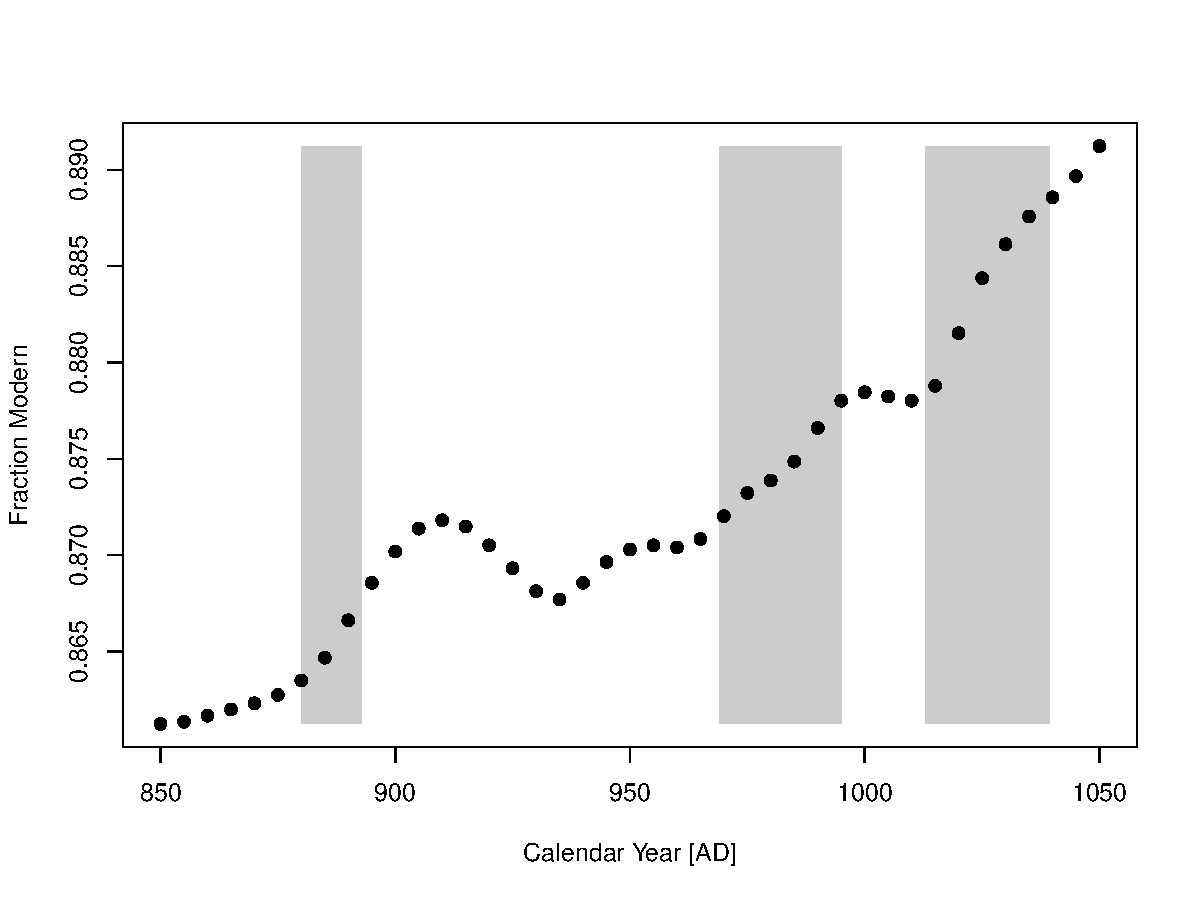
\includegraphics[height=.85\textheight]{single_obs_inf_plot2.pdf}
\end{frame}

%----------- slide --------------------------------------------------%
\begin{frame}[t]
  \frametitle{Calibration Curve}
    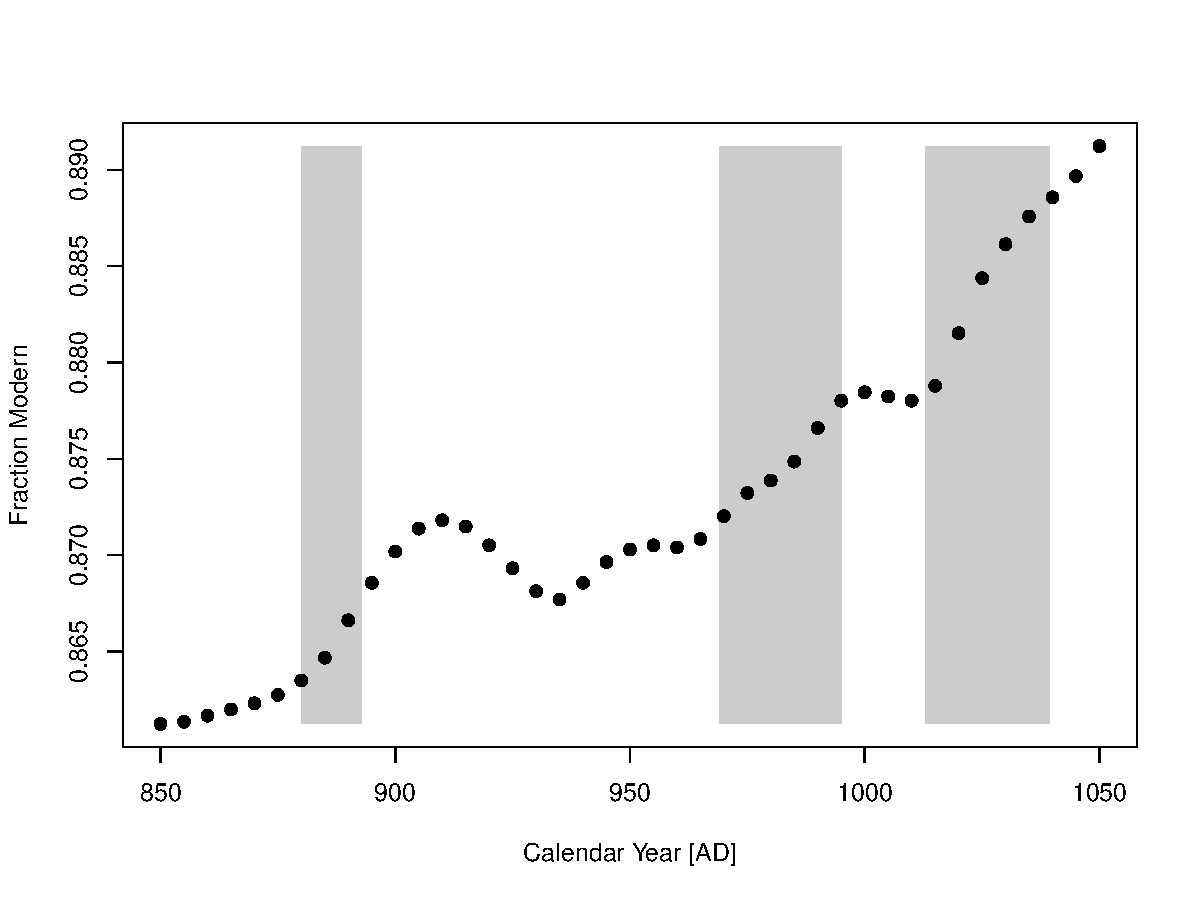
\includegraphics[height=.85\textheight]{single_obs_inf_plot2.pdf}
    \begin{textblock*}{100pt}(125pt,135pt)
      \Large $\phi_c(t)$ \normalsize
	\end{textblock*}   
\end{frame}

%----------- slide --------------------------------------------------%
\begin{frame}[t]
  \frametitle{Calibration Curve}
    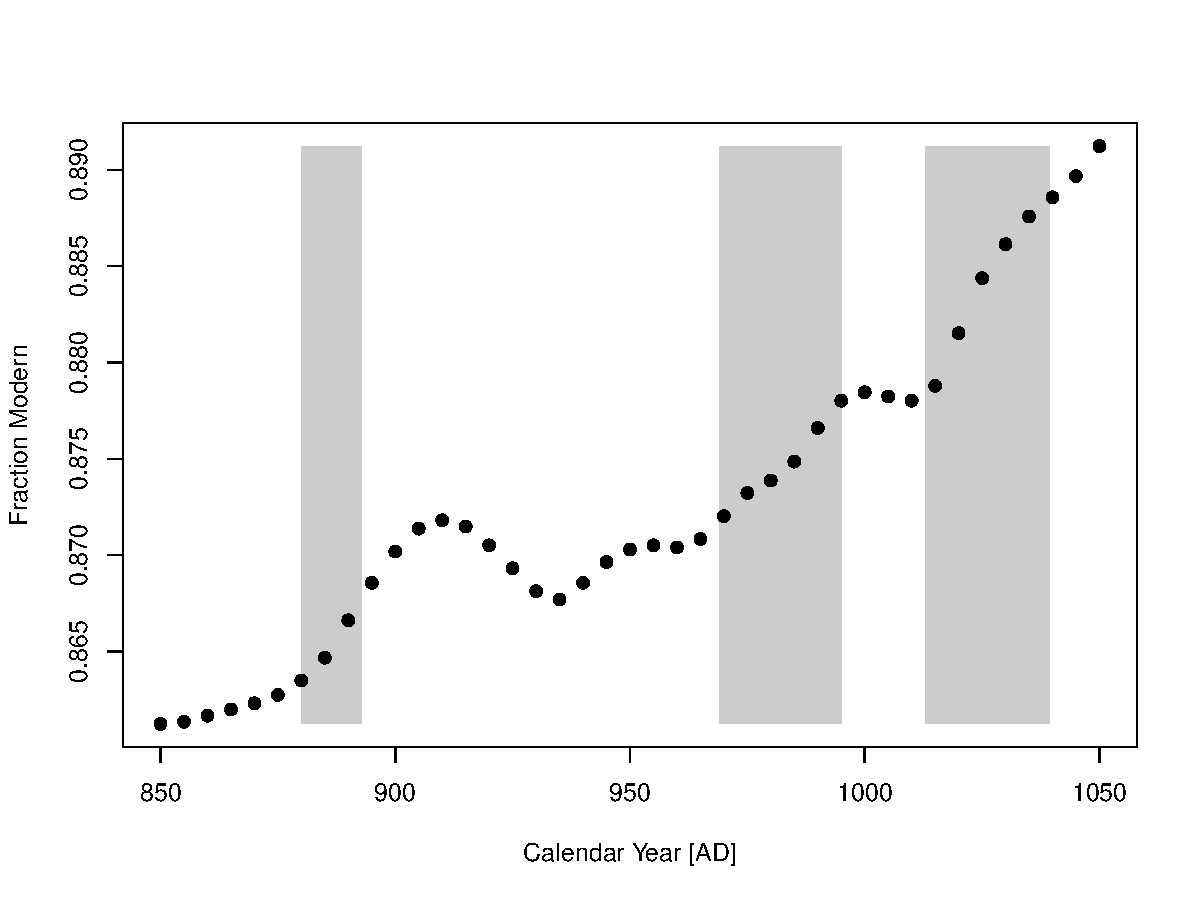
\includegraphics[height=.85\textheight]{single_obs_inf_plot2.pdf}
    \begin{textblock*}{100pt}(125pt,135pt)
      \Large $\phi_c(t)$ \normalsize
	\end{textblock*}   
    \begin{textblock*}{100pt}(125pt,185pt)
      \Large $\sigma_c(t)$ \normalsize
	\end{textblock*}   
\end{frame}

%----------- slide --------------------------------------------------%
\begin{frame}[t]
  \frametitle{Likelihood (single observation, given $t$)}
  \Large
  \begin{equation}
    \phi_m|t \sim N(\phi_c(t),\sigma^2(t))
  \end{equation}
  
  \bigskip
  
  \begin{equation}
    \sigma^2(t) = \sigma^2_m + \sigma^2_c(t)
  \end{equation}
  
  \bigskip
  
  \begin{equation}
    p(\phi_m|t) = \frac{1}{\sqrt{2\pi}\sigma(t)}\exp{(-\frac{1}{2}\frac{[\phi_m-\phi_c(t)]^2}{\sigma^2(t)})}
  \end{equation}
 
  \normalsize
\end{frame}

%----------- slide --------------------------------------------------%
\begin{frame}[t]
  \frametitle{Update (single observation, given $t$)}
  \Large
  \begin{equation}
    p(t|\phi_m) \propto p(\phi_m|t) p(t)
  \end{equation}
  \normalsize
\end{frame}

%----------- slide --------------------------------------------------%
\begin{frame}
  \frametitle{Bayesian Inference}
  \begin{center}
	\begin{equation*}
          p(\greekbf{\theta}|\mathbf{D},\greekbf{\alpha}) = \frac{p(\mathbf{D}|\greekbf{\theta}) \, p(\greekbf{\theta}|\greekbf{\alpha})}{p(\mathbf{D}|\greekbf{\alpha})}
        \end{equation*}
  \end{center}

  \pause
  \begin{center}
          \begin{equation*}
            \begin{array}{lll}
	      \greekbf{\alpha} & := & \mbox{Hyperparameter specifying priors}\\
                               &    &\\
              \greekbf{\theta} & := & \mbox{Parameter for demographic models}\\
	      \pause
                               &    &\\
              \mathbf{D}       & := & \mbox{Data}\\
                               &    &\\
            \end{array}
          \end{equation*}
  \end{center}
\end{frame}

%----------- slide --------------------------------------------------%
\begin{frame}
  \frametitle{Bayesian Inference [Gibbs, MCMC, etc.]}
  \Large
  What if $p(\greekbf{\theta}|\mathbf{D},\greekbf{\alpha})$ is hard to calculate?\\
  \pause
  \vspace{.75cm}
  Sample from the posterior distribution using well-established techniques yielding $\greekbf{\theta}_n$\\
  \pause
  \vspace{.75cm}
  $<f> = \frac{1}{N} \, \sum_{n=1}^{N} f(\greekbf{\theta_n})$\\
\end{frame}

\end{document}

%----------- slide --------------------------------------------------%
\begin{frame}
  \frametitle{Leslie Matrices}
    %\begin{block}{}
	  \begin{center}
          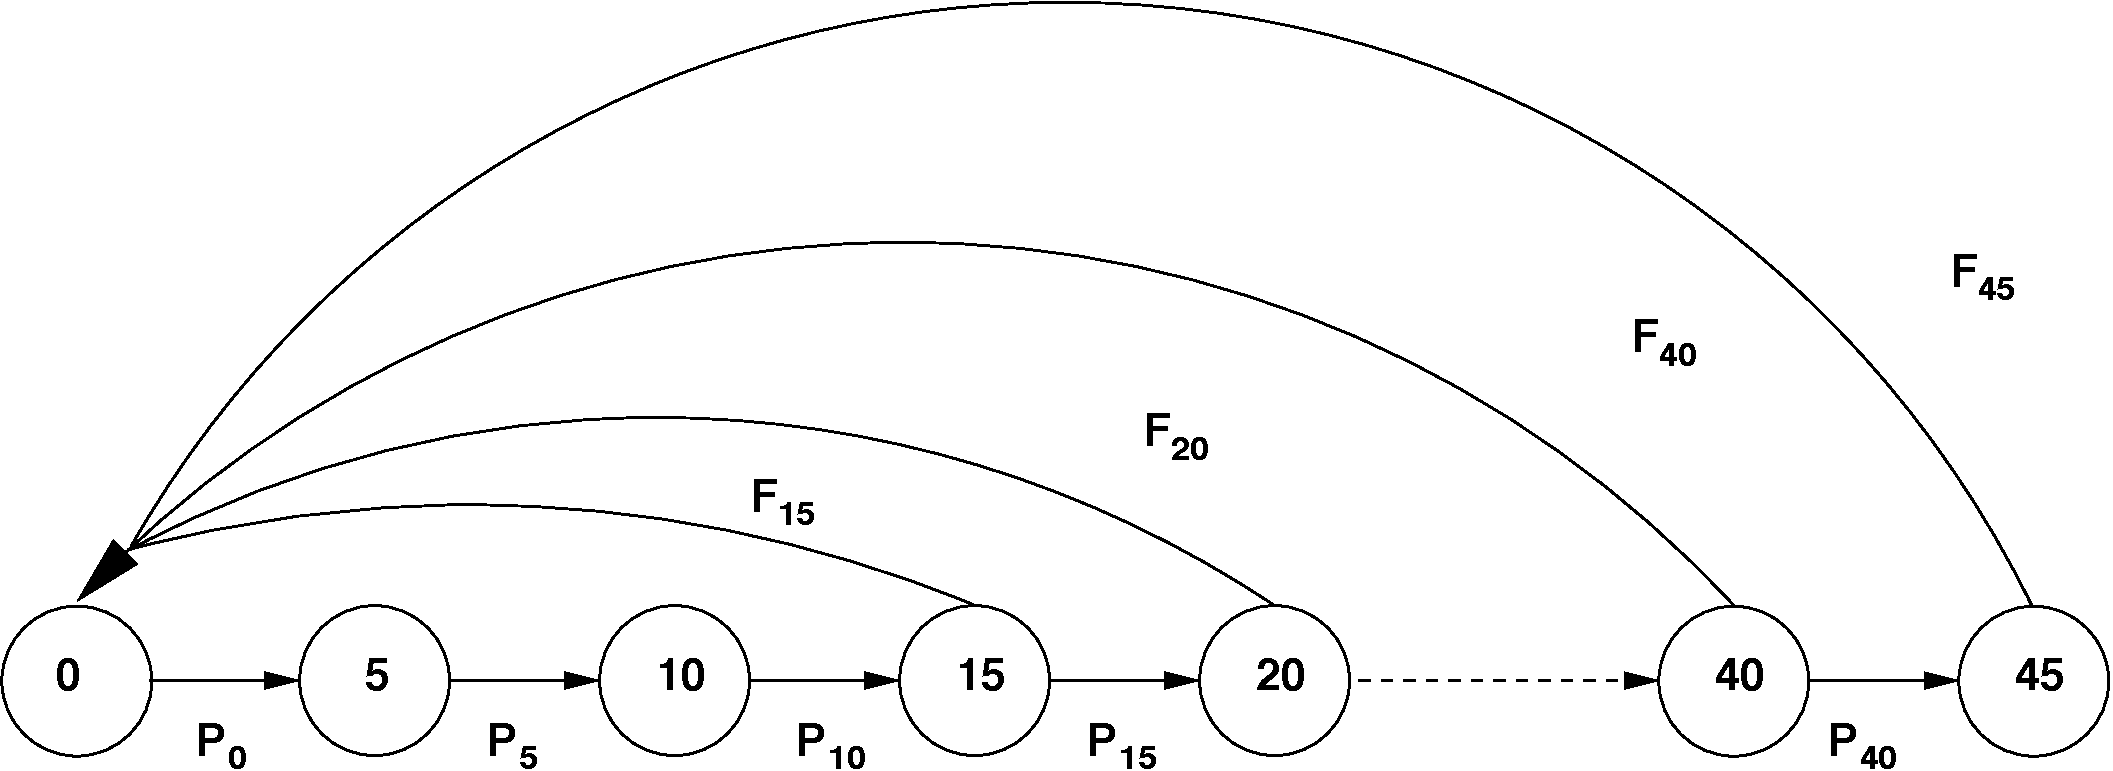
\includegraphics[width=.8\textwidth]{life-cycle.pdf}\
	  \end{center}
    %\end{block}
    \pause

    %\begin{block}{}
	  \begin{center}
	  \small
          \begin{equation*}
            \label{eq:A}
            \mathbf{A} = 
            \left( \begin{array}{cccccc}
                    F_1 & F_2 & F_3 & F_4    & \cdots  & F_{M}   \\
                    P_1 & 0   & 0   & 0      & \cdots  & 0       \\
                    0   & P_2 & 0   & 0      & \cdots  & 0       \\
                    0   & 0   & P_3 & 0      & \cdots  & 0       \\
                    0   & 0   & 0   & \ddots & \cdots  & 0       \\
                    0   & 0   & 0   & \ddots & P_{M-1} & 0
                   \end{array} \right)
          \end{equation*}
	  \end{center}
    %\end{block}

 %     $\mathbf{z}_{t+1} = \mathbf{A} \, \mathbf{z}_{t}$\\
\end{frame}

%----------- slide --------------------------------------------------%
\begin{frame}[t]
  \frametitle{Leslie Matrices}
\begin{minipage}{0\linewidth}
\begin{flushleft}                           
\begin{equation*}
      \mathbf{z}_{n+1} = \mathbf{A} \, \mathbf{z}_{n}
\end{equation*}
\pause
\begin{equation*}
	\mathbf{z}_{n} = \mathbf{A} \cdots \mathbf{A} \, \mathbf{A} \, \mathbf{z}_{0} = \mathbf{A}^t \, \mathbf{z}_{0}
\end{equation*}
\pause
\begin{equation*}
	\mathbf{z}_{n} = \mathbf{A}_n \cdots \mathbf{A}_2 \, \mathbf{A}_1 \, \mathbf{z}_{0} = {}^n_1\mathbf{Y} \, \mathbf{z}_{0}
\end{equation*}
\pause
\\
\begin{equation*}
	{}^n_1\mathbf{Y}(\greekbf{\theta}) \longrightarrow p(y,a|\greekbf{\theta})
\end{equation*}
\end{flushleft} 
\end{minipage}
\end{frame}

%----------- slide --------------------------------------------------%
\begin{frame}[t]
  \frametitle{Future Work: Radiocarbon + Age-at-Death}
    \large High growth rate implies many young people \normalsize\\
    \pause
    \bigskip
    \large Lack suitable datasets [to my knowledge]\\
    \pause
    \bigskip
    \large Need better statistical methodologies for inferring age-at-death from skeletons\\
    \pause
    \bigskip
    \large A promising PhD project, perhaps!\\
\end{frame}